\documentclass[]{article}
\usepackage{lmodern}
\usepackage{amssymb,amsmath}
\usepackage{ifxetex,ifluatex}
\usepackage{fixltx2e} % provides \textsubscript
\ifnum 0\ifxetex 1\fi\ifluatex 1\fi=0 % if pdftex
  \usepackage[T1]{fontenc}
  \usepackage[utf8]{inputenc}
\else % if luatex or xelatex
  \ifxetex
    \usepackage{mathspec}
  \else
    \usepackage{fontspec}
  \fi
  \defaultfontfeatures{Ligatures=TeX,Scale=MatchLowercase}
\fi
% use upquote if available, for straight quotes in verbatim environments
\IfFileExists{upquote.sty}{\usepackage{upquote}}{}
% use microtype if available
\IfFileExists{microtype.sty}{%
\usepackage{microtype}
\UseMicrotypeSet[protrusion]{basicmath} % disable protrusion for tt fonts
}{}
\usepackage[margin=1in]{geometry}
\usepackage{hyperref}
\hypersetup{unicode=true,
            pdftitle={Global patterns of forest autotrophic carbon fluxes},
            pdfauthor={Rebecca Banbury Morgan, Valentine Herrmann, Norbert Kunert, Ben Bond-Lamberty, Helene Muller-Landau, Kristina J. Anderson-Teixeira},
            pdfborder={0 0 0},
            breaklinks=true}
\urlstyle{same}  % don't use monospace font for urls
\usepackage{natbib}
\bibliographystyle{apalike}
\usepackage{longtable,booktabs}
\usepackage{graphicx,grffile}
\makeatletter
\def\maxwidth{\ifdim\Gin@nat@width>\linewidth\linewidth\else\Gin@nat@width\fi}
\def\maxheight{\ifdim\Gin@nat@height>\textheight\textheight\else\Gin@nat@height\fi}
\makeatother
% Scale images if necessary, so that they will not overflow the page
% margins by default, and it is still possible to overwrite the defaults
% using explicit options in \includegraphics[width, height, ...]{}
\setkeys{Gin}{width=\maxwidth,height=\maxheight,keepaspectratio}
\IfFileExists{parskip.sty}{%
\usepackage{parskip}
}{% else
\setlength{\parindent}{0pt}
\setlength{\parskip}{6pt plus 2pt minus 1pt}
}
\setlength{\emergencystretch}{3em}  % prevent overfull lines
\providecommand{\tightlist}{%
  \setlength{\itemsep}{0pt}\setlength{\parskip}{0pt}}
\setcounter{secnumdepth}{0}
% Redefines (sub)paragraphs to behave more like sections
\ifx\paragraph\undefined\else
\let\oldparagraph\paragraph
\renewcommand{\paragraph}[1]{\oldparagraph{#1}\mbox{}}
\fi
\ifx\subparagraph\undefined\else
\let\oldsubparagraph\subparagraph
\renewcommand{\subparagraph}[1]{\oldsubparagraph{#1}\mbox{}}
\fi

%%% Use protect on footnotes to avoid problems with footnotes in titles
\let\rmarkdownfootnote\footnote%
\def\footnote{\protect\rmarkdownfootnote}

%%% Change title format to be more compact
\usepackage{titling}

% Create subtitle command for use in maketitle
\providecommand{\subtitle}[1]{
  \posttitle{
    \begin{center}\large#1\end{center}
    }
}

\setlength{\droptitle}{-2em}

  \title{Global patterns of forest autotrophic carbon fluxes}
    \pretitle{\vspace{\droptitle}\centering\huge}
  \posttitle{\par}
    \author{Rebecca Banbury Morgan, Valentine Herrmann, Norbert Kunert, Ben
Bond-Lamberty, Helene Muller-Landau, Kristina J. Anderson-Teixeira}
    \preauthor{\centering\large\emph}
  \postauthor{\par}
    \date{}
    \predate{}\postdate{}
  
\usepackage{booktabs}
\usepackage{longtable}
\usepackage{array}
\usepackage{multirow}
\usepackage{wrapfig}
\usepackage{float}
\usepackage{colortbl}
\usepackage{pdflscape}
\usepackage{tabu}
\usepackage{threeparttable}
\usepackage{threeparttablex}
\usepackage[normalem]{ulem}
\usepackage{makecell}
\usepackage{xcolor}

\usepackage{float} \usepackage{caption} \captionsetup[table]{font=footnotesize} \captionsetup[figure]{font=footnotesize}

\begin{document}
\maketitle

\subsubsection{Abstract}\label{abstract}

{[}\textbf{very rough start:}{]} \ldots{}.. Here, we drew upon \#
records from the Global Forest Carbon Database (ForC), representing all
major forest types and the nine most significant forest autotrophic
carbon flux (FACF) variables, to comprehensively explore how C cycling
in mature, undisturbed forests varies with latitude and climate on a
global scale. We show that, across all FACF variables analyzed, C
cycling decreases linearly with latitude --a finding that confirms
multiple previous studies but contradicts the idea that productivity of
temperate forests rivals that of tropical forests. The FACF variables
increase in proportion to one another, with no differences in allocation
detectable at this global scale, but differed in that latitude explained
a lower proportion of variation among subsidiary fluxes (in particular,
woody aboveground productivity and belowground net primary productivity,
\(BNPP\)). Climate explained a significant proportion (\#-\#\%) of
variation in all C fluxes analyzed (less for subsidiary fluxes), with
temperature variables in general and mean annual temperature (\(MAT\))
in particular being the best predictors of FACF on this global scale.
While other climate variables (\emph{e.g.}, displayed significant
correlation with FACF, none of them improved significantly over the
explanatory power \(MAT\). The effects of temperature were modified by
moisture availability, with reduced FACF under hot and dry conditions
and sometimes under very high precipitaiton (especially for \(BNPP\)).
FACF declined with temperature seasonality, but growing season length
doesn't improve upon MAT as a predictor. Within the growing season, the
influence of climate on C cycling is smaller but still significant for a
number of carbon fluxes. These findings clarify the big picture of how
FACF varies with latitude and climate on a global scale. As we enter a
period of accelerating climatic change, understanding of the fundamental
climatic controls on FACF sets a foundation for understanding patterns
of change.

\subsubsection{Introduction}\label{introduction}

\textbf{Forests play a critical role in regulating atmospheric CO\_2 and
climate} (\textbf{Bonan}). The total amount of CO\_2 cycling through
Earth's forests each year (\emph{i.e.}, total gross primary production,
\(GPP\)) is more than five times anthropogenic fossil fuel emissions,
and net sequestration (\textasciitilde{}2.4 GtCyr\textsuperscript{-1})
offsetting roughly 30\% of these emissions \citep{pan_large_2011}. As
atmospheric carbon dioxide levels continue to rise, with consequences
for global climate, there is increasing recognition that proper
protection and management of forest resources will have an important
role to play in mitigating climate change (** REFS- e.g., IPCC 1.5C and
land reports**). Carbon fixation, allocation, and metabolism by trees
set the basis for energy and material flows in forest ecosystems and
define their interactions with Earth's changing climate.

\textbf{Forests' autotrophic carbon flux (FACF, bbl:define) influences
all organic matter stocks in ecosystems and is linked to cycling of
energy, water, and nutrients} (\textbf{REFS; \emph{Piao et al. 2010.
Forest annual carbon cost: a global‐scale analysis of autotrophic
respiration. Ecology 91(3), 652-661Ƴ} }). Forest productivity sets the
energy ultimately available to heterotrophic organisms (including
microbes), in turn influencing their abundance (\textbf{REFS}) and
possibly diversity
(\href{https://www.annualreviews.org/doi/abs/10.1146/annurev.ecolsys.30.1.257}{Waide
et al. 2009}\textbf{REFS})--but probably not individual metabolic rate
(\textbf{Anderson \& Jetz 2005, but check more recent literature}).
However, our ability to draw general macroscopic conclusions regarding
global variation in multiple productivity variables with respect to
climate has been limited in that these analyses often mix forests that
vary in stand age, disturbance history, and/or management status; do not
always sufficiently parse related variables (\emph{e.g.}, combining net
primary productivity records with and without belowground components);
and typically consider only one or a few variables at a time.

\textbf{The productivity of forests varies with latitude}, showing a
general trend of decreasing productivity with latitude
\citep{beer_terrestrial_2010, jung_global_2011}. Studies agree that
productivity is lowest in the boreal regions, and increases into the
temperate regions
\citep{luyssaert_co_2007, huston_global_2009, beer_terrestrial_2010, jung_global_2011}.
However, evidence is inconclusive on whether productivity continues to
increase into the tropics, or whether it plateaus in temperate regions.
Evidence for this is further complicated by the fact that different
studies use different measures of productivity to explore these
relationships. For example, modelling of global terrestrial ecosystem
gross primary productivity (GPP) through upscaling and calibration of
eddy flux measurements indicates that GPP peaks in tropical forests
\citep{beer_terrestrial_2010, jung_global_2011};\href{https://onlinelibrary.wiley.com/doi/epdf/10.1111/gcb.14729}{Bagdley
et al. 2019}). This is corroborated by analysis of site-level GPP
measurements, which appear to reach their highest levels in tropical
forests \citep{luyssaert_co_2007}. In contrast, there is evidence that
the highest values of net primary productivity (NPP) may be found in
temperate forests \citep{luyssaert_co_2007, huston_global_2009},
although other studies find NPP is highest in the tropics, showing a
decrease with latitude \citep{simova_enigma_2017}. Other studies have
chosen to focus exclusively on above-ground net primary productivity
(ANPP), finding evidence of a weak negative relationship between ANPP
and latitude \citep{huston_global_2009, gillman_latitude_2015}.

\textbf{Climate is a significant driver of productivity across broad
spatial scales} \citep{cleveland_relationships_2011}. The majority of
studies have focused on exploring the relationships between productivity
and mean annual temperature (MAT) and mean annual precipitation (MAP),
as the most commonly reported site-level climate variables. These
variables have the advantage that they describe broad trends in
temperature and water availability, and therefore capture a lot of
global-scale variation in climate. There is strong evidence that both
MAT and MAP show significant positive relationships with productivity
\citep{chu_does_2016}. However, as with latitude, the shape of those
relationships is not always clear, and, again, is complicated by the use
of different measures of productivity across studies. Various measures
of primary productivity saturate at high levels of MAP, though the
saturation points identified vary from 1500mm \citep{luyssaert_co_2007}
up to 2445mm MAP \citep{schuur_productivity_2003}. Studies of the
influence of MAT on productivity are less conclusive. Luyssaert et al.
\citeyearpar{luyssaert_co_2007} examined GPP and NPP and found that,
while GPP increases linearly with MAT, NPP saturates at around
10\(^\circ\)C MAT. In contrast, Larjavaara and Muller-Landau
\citeyearpar{larjavaara_temperature_2012}, find that increases in GPP
saturate at approximately 25\(^\circ\)C MAT, while Schuur
\citeyearpar{schuur_productivity_2003} shows that NPP increases linearly
with temperature. bbl:maybe remove following sentences The influence of
these climate variables on productivity is further complicated by the
possibility of interactive effects occurring between them. Taylor et al.
\citeyearpar{taylor_temperature_2017} showed that increased MAP had a
negative effect at low MAT, but a positive effect at high levels of MAT,
and vice versa, suggesting that both temperature and water availability
are important in explaining productivity.

\textbf{Primary productivity can be influenced by many other factors as
well}, which often act across a range of scales, and may show
interactive effects with each other
\citep{cleveland_relationships_2011}. On a local scale, stand age
\citep{litton_carbon_2007, gillman_latitude_2015}, biodiversity (Liang
et al. 2019. Positive biodiversity-productivity relationship predominant
in global forests. Science 354, Issue 6309, aaf8957), management
\citep{simova_enigma_2017}; nutrient availability
\citep{aragao_above-_2009}; and altitude
\citep{girardin_net_2010, malhi_variation_2017} all impact forest
productivity. On a global scale, we expect that productivity is most
strongly influenced by broad climatic gradients. There is evidence that
productivity also responds to variables such as cloud cover
\citep{taylor_temperature_2017}, solar radiation
\citep{fyllas_solar_2017}, and potential evapotranspiration
\citep{kerkhoff_plant_2005} in potentially significant ways.
Furthermore, MAT and MAP are very coarse measures of climate, and so
fail to capture much variation in climate on an intra-annual scale,
including the effects of factors such as growing season length, number
of frost-free days, temperature seasonality, and dry season length. Some
studies have suggested that the apparently strong relationship between
MAT and productivity is actually a factor of the correlation between MAT
and growing season length
\citep{kerkhoff_plant_2005, malhi_productivity_2012, michaletz_convergence_2014, michaletz_drivers_2018}.
Kerkhoff et al. \citeyearpar{kerkhoff_plant_2005} and Michaletz et al.
\citeyearpar{michaletz_convergence_2014} find that, within the growing
season, there is no significant relationship between productivity and
MAT, indicating that the effect of temperature is due to increased
length of growing season, rather than an inherent influence of
temperature on productivity.

\textbf{The recent development of a global forest carbon database
synthesizing multiple variables and including records of stand history
(ForC;
\citep{anderson-teixeira_carbon_2016, anderson-teixeira_forc:_2018})
opens up the possibility for a standardized analysis of global scale
variation} in multiple components of forest productivity and the
principle climatic drivers of these patterns. In order to approach these
broad and complex issues, we simplify the major gaps in our knowledge to
five broad hypotheses and corresponding specific predictions (Table 1).
First, we ask how forest autotrophic carbon fluxes (FACF) vary with
latitude. We then test how these fluxes relate to MAT and MAP, and
additionally how they respond to other, less well studied, climate
variables. We finally consider the relationship between FACF and
seasonality, considering the role of seasonality in explaining variation
in carbon fluxes, and the influence of climate on FACF per month of the
growing season. We use a comprehensive global database of forest carbon
fluxes to explore the above questions for nine carbon fluxes, allowing
for an in-depth exploration of the effect of climate on global
productivity.

\renewcommand{\arraystretch}{2}

\begin{landscape}\begin{table}[!h]

\caption{\label{tab:unnamed-chunk-4}**Summary of hypotheses, corresponding specific predictions, and results.** Direction of significant relationships is indicated by '+' and '-', and  shape is summarized as linear (L), concave up (CU), and concave down (CD). 'n.s.' indicates that the relationship is not signficant.}
\centering
\resizebox{\linewidth}{!}{
\fontsize{12}{14}\selectfont
\begin{tabular}{>{\raggedright\arraybackslash}p{10cm}>{\raggedright\arraybackslash}p{5cm}>{\raggedright\arraybackslash}p{1.8cm}>{\raggedright\arraybackslash}p{1.8cm}>{\raggedright\arraybackslash}p{1.8cm}>{\raggedright\arraybackslash}p{1.8cm}>{\raggedright\arraybackslash}p{1.8cm}>{\raggedright\arraybackslash}p{1.8cm}>{\raggedright\arraybackslash}p{1.8cm}>{\raggedright\arraybackslash}p{1.8cm}>{\raggedright\arraybackslash}p{1.8cm}>{\raggedright\arraybackslash}p{1.8cm}>{\raggedright\arraybackslash}p{1.8cm}}
\toprule
\multicolumn{1}{c}{ } & \multicolumn{1}{c}{ } & \multicolumn{1}{c}{ } & \multicolumn{9}{c}{Forest autotrophic carbon fluxes (FACF)} & \multicolumn{1}{c}{ } \\
\cmidrule(l{3pt}r{3pt}){4-12}
Hypotheses \& Specific Predictions & Related references & Overall & GPP & NPP & ANPP & BNPP & ANPP foliage & ANPP woody stem & BNPP fine root & R auto root & R auto & Support\\
\midrule
\addlinespace[1em]
\hline
\multicolumn{1}{l}{\textbf{H1. FACFs decrease linearly with latitude, and in constant proportion.}}\\
\hspace{1em}1.1. FACFs decrease linearly with latitude (L-) & Luyssaert et al. (2007) & yes & yes & yes & yes & yes & yes & yes & yes & yes & yes & Fig. 2-3\\
\hspace{1em}1.1.alt. FACFs are similar in tropical and temperate forests, but lower in boreal regions (CD-) & Gillman et al. (2015); Simova and Storch (2017) & no & no & no & no & no & no & no & no & no & no & Fig. 2-3\\
\hspace{1em}1.2. Allocation of GPP to subsidiary fluxes varies with latitude & Litton et al. (2007); DeLucia et al. (2007) & no & - & no & no & no & no & no & no & - & - & \\
\addlinespace[1em]
\hline
\multicolumn{1}{l}{\textbf{H2. FACFs increase with MAT, with an interactive effect of MAP.}}\\
\hspace{1em}2.1. FACFs increase linearly with MAT (L+) & Schuur (2003) & yes & yes & yes & yes & yes & yes & yes & yes & yes & yes & Fig. 5\\
\hspace{1em}2.2. FACFs increase with precipitation but saturate or decrease at very high levels (CD+) & Luyssaert et al. (2007); Schuur (2003) & yes & yes & yes & yes & yes & yes & n.s. & L+ & L+ & yes & Fig. 5\\
\hspace{1em}2.3. There is a postive interaction between temperature and precipitation (I+) & Taylor et al. (2016) & (yes) & yes & L+ & yes & L- & L+ & yes & L- & yes & yes & Fig. 4\\
\addlinespace[1em]
\hline
\multicolumn{1}{l}{\textbf{H3. FACFs are strongly correlated with other annual climate variables.}}\\
\hspace{1em}3.1. FACFs increases with PET, but saturates or decreases at high levels (CD+) &  & (yes) & yes & yes & yes & yes & L+ & yes & L+ & yes & L+ & Fig. 5\\
\hspace{1em}3.2. FACFs increase with vapour pressure deficit, but saturate or decrease at high levels (CD+) &  & (yes) & yes & yes & yes & yes & yes & yes & L+ & yes & yes & Fig. 5\\
\hspace{1em}3.3. FACFs increase linearly with solar radiation (L+) &  & (yes) & yes & yes & yes & CD+ & yes & CD+ & yes & n.s. & yes & \\
\addlinespace[1em]
\hline
\multicolumn{1}{l}{\textbf{H4. FACFs are reduced under seasonal climates.}}\\
\hspace{1em}4.1. FACFs decrease linearly with temperature seasonality (L-) &  & yes & CU+ & CU+ & CU+ & yes & yes & yes & yes & CU+ & CU+ & Fig. 5\\
\hspace{1em}4.2. FACFs decrease linearly with  precipitation seasonality (L-) &  & no & n.s. & n.s. & n.s. & n.s. & n.s. & n.s. & n.s. & n.s. & n.s. & \\
\hspace{1em}4.3. FACFs increase linearly with growing season length (L+) & Malhi (2012); Michaletz et al. (2014); Chu et al. (2016) & yes & yes & yes & yes & yes & yes & yes & yes & yes & yes & Fig. 5\\
\hspace{1em}4.4. Growing season length is a better predictor of FACFs than MAT & Michaletz et al. (2014); Chu et al. (2016) & no & no & no & no & no & no & no & no & no & no & \\
\addlinespace[1em]
\hline
\multicolumn{1}{l}{\textbf{H5. Considering only growing season months, FACF correlates with climatic drivers.}}\\
\hspace{1em}5.1. Increase with temperature (L+) & Michaletz et al. (2014) & (mixed) & n.s. & n.s. & yes & n.s. & yes & n.s. & n.s. & n.s. & n.s. & \\
\hspace{1em}5.2. Increase with PET (L+) &  & (yes) & yes & yes & n.s. & yes & n.s. & yes & yes & n.s. & n.s. & \\
\hspace{1em}5.3. Increase with precipitation (L+) &  & no & n.s. & n.s. & yes & n.s. & yes & n.s. & n.s. & n.s. & n.s. & \\
\hspace{1em}5.4. Increase with solar radiation (L+) &  & (mixed) & yes & yes & n.s. & yes & n.s. & n.s. & yes & n.s. & n.s. & \\
\bottomrule
\end{tabular}}
\end{table}
\end{landscape}

\subsubsection{Materials and Methods}\label{materials-and-methods}

Analyses were conducted on data contained in the open-access ForC
database
\citep{anderson-teixeira_carbon_2016, anderson-teixeira_forc:_2018}.
This database contains records of field-based measurements of forest
carbon stocks and annual fluxes, compiled from original publications and
existing data compilations and databases. Associated data, such as stand
age, measurement methodologies, and disturbance history, are also
included. The database was significantly expanded since the publication
of \citep{anderson-teixeira_forc:_2018} through integration with the
Global Database of Soil Respiration Database
\citep{bond-lamberty_global_2010}. Additional targeted literature
searches were conducted to identify any further available data on
primary productivity, with particular focus on mature forests in
temperate and boreal regions. ForC currently contains 29730 records from
4979 plots, representing 20 distinct ecozones across all forested
biogeographic and climate zones. We used ForC v3.0, archived on Zenodo
with DOI 10.5281/zenodo.3403855.

\begin{figure}[H]
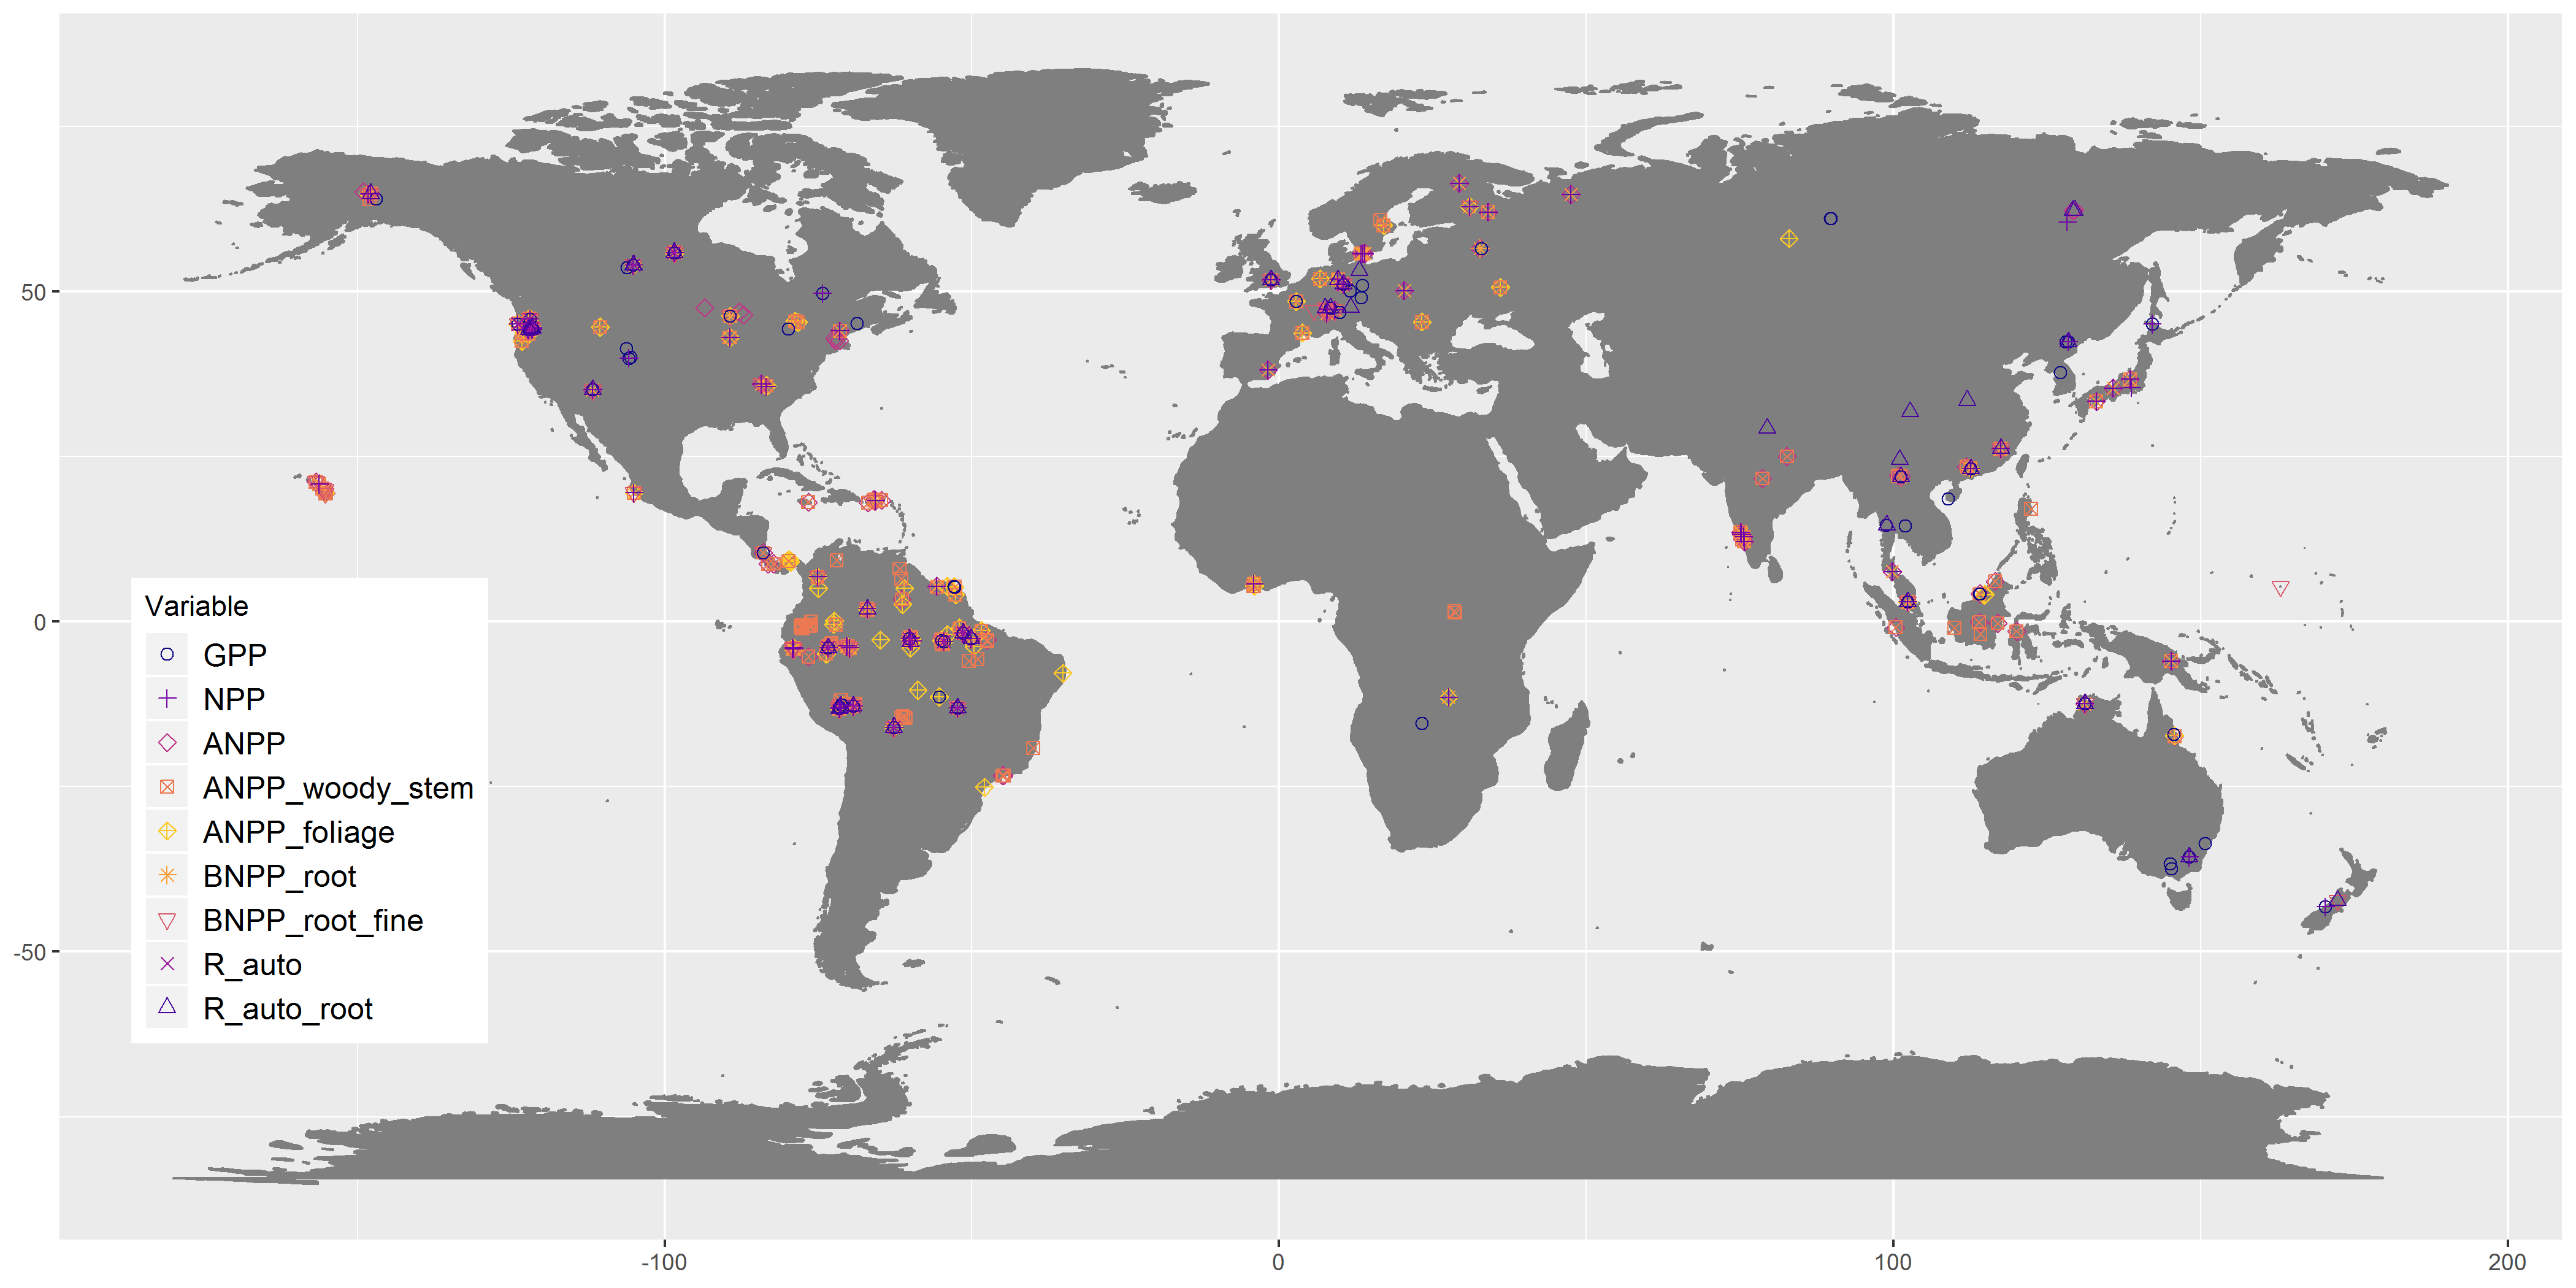
\includegraphics[width=1\linewidth]{distribution_all_variables} \caption{Map showing all data used in the analysis, coded by variable}\label{fig:unnamed-chunk-5}
\end{figure}

\emph{Data selection.} Over 50 variables of forest carbon stocks and
annual fluxes are represented in the ForC database; this analysis
focussed on measures of primary productivity. Table 1 contains details
of the variables selected for analysis.

\begin{longtable}[]{@{}llllll@{}}
\caption{Definitions and sample sizes of variables used in analysis.
Geographic areas group geographically proximate sites, defined using a
hierarchical cluster analysis on the distance matrix of the sites, and a
cutoff of 25km.}\tabularnewline
\toprule
\begin{minipage}[b]{0.14\columnwidth}\raggedright\strut
Variable\strut
\end{minipage} & \begin{minipage}[b]{0.19\columnwidth}\raggedright\strut
Definition\strut
\end{minipage} & \begin{minipage}[b]{0.13\columnwidth}\raggedright\strut
Components included\strut
\end{minipage} & \begin{minipage}[b]{0.23\columnwidth}\raggedright\strut
Methodologies used\strut
\end{minipage} & \begin{minipage}[b]{0.07\columnwidth}\raggedright\strut
Number of records\strut
\end{minipage} & \begin{minipage}[b]{0.07\columnwidth}\raggedright\strut
Number of geographic areas\strut
\end{minipage}\tabularnewline
\midrule
\endfirsthead
\toprule
\begin{minipage}[b]{0.14\columnwidth}\raggedright\strut
Variable\strut
\end{minipage} & \begin{minipage}[b]{0.19\columnwidth}\raggedright\strut
Definition\strut
\end{minipage} & \begin{minipage}[b]{0.13\columnwidth}\raggedright\strut
Components included\strut
\end{minipage} & \begin{minipage}[b]{0.23\columnwidth}\raggedright\strut
Methodologies used\strut
\end{minipage} & \begin{minipage}[b]{0.07\columnwidth}\raggedright\strut
Number of records\strut
\end{minipage} & \begin{minipage}[b]{0.07\columnwidth}\raggedright\strut
Number of geographic areas\strut
\end{minipage}\tabularnewline
\midrule
\endhead
\begin{minipage}[t]{0.14\columnwidth}\raggedright\strut
\(GPP\)\strut
\end{minipage} & \begin{minipage}[t]{0.19\columnwidth}\raggedright\strut
Annual gross primary production; annual uptake of carbon dioxide by an
ecosystem\strut
\end{minipage} & \begin{minipage}[t]{0.13\columnwidth}\raggedright\strut
NA\strut
\end{minipage} & \begin{minipage}[t]{0.23\columnwidth}\raggedright\strut
Flux partitioning of eddy covariance\strut
\end{minipage} & \begin{minipage}[t]{0.07\columnwidth}\raggedright\strut
243\strut
\end{minipage} & \begin{minipage}[t]{0.07\columnwidth}\raggedright\strut
49\strut
\end{minipage}\tabularnewline
\begin{minipage}[t]{0.14\columnwidth}\raggedright\strut
\(NPP\)\strut
\end{minipage} & \begin{minipage}[t]{0.19\columnwidth}\raggedright\strut
Annual net primary production; the component of GPP that is stored in
plant tissue; \(GPP - R_{auto}\)\strut
\end{minipage} & \begin{minipage}[t]{0.13\columnwidth}\raggedright\strut
Foliage, branch, stem, coarse root and fine root\strut
\end{minipage} & \begin{minipage}[t]{0.23\columnwidth}\raggedright\strut
Direct measurement of annual increments of components\strut
\end{minipage} & \begin{minipage}[t]{0.07\columnwidth}\raggedright\strut
92\strut
\end{minipage} & \begin{minipage}[t]{0.07\columnwidth}\raggedright\strut
42\strut
\end{minipage}\tabularnewline
\begin{minipage}[t]{0.14\columnwidth}\raggedright\strut
\(ANPP\)\strut
\end{minipage} & \begin{minipage}[t]{0.19\columnwidth}\raggedright\strut
Aboveground net primary production\strut
\end{minipage} & \begin{minipage}[t]{0.13\columnwidth}\raggedright\strut
Foliage, stem, and optionally branch\strut
\end{minipage} & \begin{minipage}[t]{0.23\columnwidth}\raggedright\strut
Direct measurement of annual increments of components\strut
\end{minipage} & \begin{minipage}[t]{0.07\columnwidth}\raggedright\strut
256\strut
\end{minipage} & \begin{minipage}[t]{0.07\columnwidth}\raggedright\strut
80\strut
\end{minipage}\tabularnewline
\begin{minipage}[t]{0.14\columnwidth}\raggedright\strut
\(ANPP_{foliage}\)\strut
\end{minipage} & \begin{minipage}[t]{0.19\columnwidth}\raggedright\strut
Net primary production of foliage\strut
\end{minipage} & \begin{minipage}[t]{0.13\columnwidth}\raggedright\strut
Foliage\strut
\end{minipage} & \begin{minipage}[t]{0.23\columnwidth}\raggedright\strut
Direct measurement of litterfall, correcting for changes in leaf biomass
when measured\strut
\end{minipage} & \begin{minipage}[t]{0.07\columnwidth}\raggedright\strut
98\strut
\end{minipage} & \begin{minipage}[t]{0.07\columnwidth}\raggedright\strut
49\strut
\end{minipage}\tabularnewline
\begin{minipage}[t]{0.14\columnwidth}\raggedright\strut
\(ANPP_{woody-stem}\)\strut
\end{minipage} & \begin{minipage}[t]{0.19\columnwidth}\raggedright\strut
Net primary production of woody stems\strut
\end{minipage} & \begin{minipage}[t]{0.13\columnwidth}\raggedright\strut
Woody stems\strut
\end{minipage} & \begin{minipage}[t]{0.23\columnwidth}\raggedright\strut
Direct measurement of stem growth increment\strut
\end{minipage} & \begin{minipage}[t]{0.07\columnwidth}\raggedright\strut
264\strut
\end{minipage} & \begin{minipage}[t]{0.07\columnwidth}\raggedright\strut
96\strut
\end{minipage}\tabularnewline
\begin{minipage}[t]{0.14\columnwidth}\raggedright\strut
\(BNPP_{root}\)\strut
\end{minipage} & \begin{minipage}[t]{0.19\columnwidth}\raggedright\strut
Belowground net primary production\strut
\end{minipage} & \begin{minipage}[t]{0.13\columnwidth}\raggedright\strut
Coarse and fine roots\strut
\end{minipage} & \begin{minipage}[t]{0.23\columnwidth}\raggedright\strut
Direct measurement of one or more of: fine root turnover, soil cores,
root ingrowth cores, minirhizotrons; indirect estimates of coarse roots
using allometries based on aboveground stem increment measures\strut
\end{minipage} & \begin{minipage}[t]{0.07\columnwidth}\raggedright\strut
101\strut
\end{minipage} & \begin{minipage}[t]{0.07\columnwidth}\raggedright\strut
48\strut
\end{minipage}\tabularnewline
\begin{minipage}[t]{0.14\columnwidth}\raggedright\strut
\(BNPP_{fine.root}\)\strut
\end{minipage} & \begin{minipage}[t]{0.19\columnwidth}\raggedright\strut
Net primary production of fine roots\strut
\end{minipage} & \begin{minipage}[t]{0.13\columnwidth}\raggedright\strut
Fine roots\strut
\end{minipage} & \begin{minipage}[t]{0.23\columnwidth}\raggedright\strut
Direct measurement of one or more of: minirhizotrons, fine root
turnover, soil cores, root ingrowth cores\strut
\end{minipage} & \begin{minipage}[t]{0.07\columnwidth}\raggedright\strut
88\strut
\end{minipage} & \begin{minipage}[t]{0.07\columnwidth}\raggedright\strut
41\strut
\end{minipage}\tabularnewline
\begin{minipage}[t]{0.14\columnwidth}\raggedright\strut
\(R_{auto}\)\strut
\end{minipage} & \begin{minipage}[t]{0.19\columnwidth}\raggedright\strut
Annual autotrophic respiration, including above- and belowground
components\strut
\end{minipage} & \begin{minipage}[t]{0.13\columnwidth}\raggedright\strut
Foliage, stem, and root\strut
\end{minipage} & \begin{minipage}[t]{0.23\columnwidth}\raggedright\strut
Chamber measurements of component gas exchange\strut
\end{minipage} & \begin{minipage}[t]{0.07\columnwidth}\raggedright\strut
22\strut
\end{minipage} & \begin{minipage}[t]{0.07\columnwidth}\raggedright\strut
13\strut
\end{minipage}\tabularnewline
\begin{minipage}[t]{0.14\columnwidth}\raggedright\strut
\(R_{root}\)\strut
\end{minipage} & \begin{minipage}[t]{0.19\columnwidth}\raggedright\strut
Annual root respiration\strut
\end{minipage} & \begin{minipage}[t]{0.13\columnwidth}\raggedright\strut
Coarse and fine roots\strut
\end{minipage} & \begin{minipage}[t]{0.23\columnwidth}\raggedright\strut
\emph{Measurement of root gas exchange, root exclusion from soil
respiration chambers}\strut
\end{minipage} & \begin{minipage}[t]{0.07\columnwidth}\raggedright\strut
64\strut
\end{minipage} & \begin{minipage}[t]{0.07\columnwidth}\raggedright\strut
26\strut
\end{minipage}\tabularnewline
\bottomrule
\end{longtable}

A subset of the ForC database was generated for the purposes of this
analysis, in order to control for data quality and remove biasing
factors. Since management can alter observed patterns of primary
productivity \citep{simova_enigma_2017}, sites were excluded from
analysis if they were managed, defined as plots that were planted,
managed as plantations, irrigated, fertilised or including the term
``managed'' in their site description. Sites that had experienced
significant disturbance were also excluded. Disturbances that justified
site exclusion were major cutting or harvesting, and/or burning,
flooding, drought and storm events with site mortality
\textgreater{}10\% of trees. Grazed sites were retained.\\
There is evidence that stand age influences patterns of primary
productivity and carbon allocation in forest ecosystems, and can
confound relationships between latitude and primary productivity
\citep{de_lucia_forest_2007, gillman_latitude_2015}. To reduce any
biasing effects of stand age, stands under 100 years of age were
excluded from analysis. Sites for which stand age was unknown were
excluded from analysis.

\emph{Methodological consistency.} The data in ForC is derived from a
range of studies, often employing different methods. For this reason,
criteria were introduced to standardise for differences in methodology.
Where data was based on forest plot census measurements, studies which
used a minimum diameter at breast height (DBH) measure of
\textgreater{}10cm were excluded from analysis. It would be preferable
to standardise by minimum area sampled; however x\% of plots in the
database are 1 ha or under in size; excluding these plots would place
significant constraints on sample size.

As discussed above, estimates of \(NPP\), \(ANPP\), and \(BNPP\) are
generated through summing measurements of their component parts. Since
the components included in productivity estimates vary between studies,
estimates of productivity were classified within the ForC database
according to their components, and then filtered for analysis. Estimates
of NPP were selected if they included foliage, branch, stem, coarse
root, and fine root. Measures of NPP which included additional
components, including understorey, volatile organic compounds (VOCs),
exudates, estimates of NPP lost to herbivory, and the NPP of
reproductive structures, were excluded. Estimates of ANPP were selected
if they included foliage, stem growth and optionally branch turnover.
Any measures of primary productivity where components were unknown were
excluded from analysis.

\emph{Climate datasets.} Where site-level data on mean annual
temperature, mean annual precipitation, and latitude were available in
the primary literature, this data was compiled and entered directly into
the ForC database. Based on the geographic co-ordinates for each site,
data on a further 11 climate variables was extracted from five
open-access climate datasets: WorldClim \citep{hijmans_very_2005},
WorldClim2 \citep{fick_worldclim_2017}, the Climate Research Unit (CRU)
time-series dataset v. 4.03 \citep{harris_updated_2014}, the Global
Aridity Index and Potential Evapotranspiration Climate Database
\citep{trabucco_global_2018}, and TerraClimate
\citep{abatzoglou_terraclimate_2018} (see Supplementary Information S1
for details of climate variables). Where site-level data was missing for
mean annual temperature and/or mean annual precipitation, data was
extracted from the WorldClim dataset.

Additionally, two climate variables were derived from the above
datasets: maximum vapour pressure deficit, defined as the vapour
pressure deficit of the month with the largest deficit; and water stress
months, defined as the number of months annually where precipitation was
lower than potential evapotranspiration.

\emph{Length of growing season.} Growing season months were defined as
months with mean minimum temperature \textgreater{} 0.5\(^\circ\)C.
Growing season months were initially calculated following methods used
by Kerkhoff et al. (2005), which additionally required that growing
season months had a moisture index, defined as (MAT - PET)/PET,
\textgreater{} -0.95. Michaletz et al. (2014) included an equivalent
requirement in their calculation of growing season length. However, we
found that including this requirement had no effect on the estimates of
growing season length, and so chose to exclude it.

Monthly data for PET, precipitation, and temperature was downloaded from
the Climate Research Unit (CRU) time-series dataset v 4.03
\citep{harris_updated_2014}, and for solar radiation from WorldClim2
\citep{fick_worldclim_2017}, and used to calculate mean monthly PET,
precipitation, temperature and solar radiation during the growing
season. Total growing season precipitation and solar radiation were also
calculated.

\emph{Model specification.} The effects of climate and latitude on
primary productivity were analysed using mixed effects models using the
package `lme4' \citep{bates_fitting_2015} in R v.3.5.1
\citep{r_core_team_r:_2018}. The effect of each extracted climate
variable on each measure of primary productivity was modelled by
specifying the climate variable as a fixed effect. For each climate
variable, three models were specified: a null model; a model with the
climate variable as a linear term; and a model with the climate variable
as a polynomial term. AIC values were calculated for the models and used
to select the best model. If the best model included a polynomial term,
the shape of the polynomial relationship was considered. If the shape of
the relationship \emph{made biological sense}, and was a significant
improvement on the linear relationship (deltaAIC \textgreater{}2), we
accepted the polynomial as the best model. If not, we ran the linear
model as the final model. \(R^2\) values were calculated for the best
model. All \(R^2\) values presented here are marginal \(R^2\) values,
and refer to the proportion of variation explained by only the fixed
effects, unless otherwise specified. In addition, slope coefficients
were calculated for the linear models.

Because the magnitude of fluxes varies significantly, in order to
facilitate comparisons between regression models for each flux, data for
each flux was scaled, to give the data a mean of 0 and standard
deviation of 1. As each data set was scaled separately, this does not
allow for statistical comparisons of slope values, but does assist in
visualising the data.

To test for a potential influence of altitude, models were also run with
site altitude included as a second fixed effect. These models were
compared against models with no altitude term, and AIC values calculated
to identify whether inclusion of altitude as a term improved the models.
Including altitude had a very small effect on most models, with the
difference in AIC values between models including and excluding altitude
often being \textless{}2, suggesting the models are very similar in
their explanatory power. As a result, it was decided to present results
only from models do not include altitude as a fixed term.

Within the ForC database, sites within 25km\textsuperscript{2} of each
other are clustered into geographic areas. To account for correlations
in measurements between tightly clustered sites, a random effect was
specified as plot nested within geographic area. \emph{Data from the
temperate regions was heavily skewed towards studies from the old-growth
forests of the Pacific Northwest.} These forests have very high
productivity, and so to ensure that results were not unduly influenced
by geographic sampling bias, we tried a version of the model where data
were weighted according to forested land area within each Koeppen
climate zone. Results were similar between the weighted and unweighted
model, so, to avoid problems of over-fitting, the weighted model was
dropped, and results from this are not presented here.

Models were run for total annual productivity against annual climate
variables, and for monthly growing season productivity, defined as total
productivity/length of growing season, against growing season climate
variables. For analyses on data within the growing season, only linear
models were specified.

To investigate the potential interactive effects of climate variables on
carbon fluxes, multivariate models were also specified. To ensure that
models were biologically meaningful, the terms included in the models
tested built on results from the univariate models. Modelling of
individual climate variables identified that the best predictors of
carbon fluxes were variables related to temperature. We therefore
decided to include mean annual temperature as a term in all multivariate
models. We first modelled the interaction effect between mean annual
temperature and mean annual precipitation, in order to capture climate
variation along the axes of temperature and water availability. Models
were tested for a significant interactive effect and a significant
additive effect. We then explored whether any other climate variable, in
combination with mean annual temperature, could significantly improve on
the combination of mean annual temperature and mean annual
precipitation. In specifying the range of models to test, climate
variables which were strongly correlated with temperature were dropped,
in order to capture the greatest range of variation in climate. For each
possible pairing of climate variables, two models were specified: a
model with the two climate variables showing an additive effect; and a
model with the two climate variables showing an interactive effect. As
before, plot nested within geographic area was included as a random
effect. Altitude was not considered. AIC values were calculated for the
models, and used to compare models. Models were considered to be
significantly better than the baseline MAT*MAP model if:\\
i) the AIC value of the model was smaller than the AIC value of the
baseline model by \textgreater{}2\\
ii) the r-squared value of the model was larger than the r-squared value
of the baseline model by \textgreater{}5

\emph{Validating models of component fluxes.} Comparison of component
fluxes is based on the assumption that components sum accurately to
estimates of larger fluxes. To test this, components of larger fluxes
were regressed against latitude, and the models used to generate a
series of point estimates along lines of best fit for each component.
The point estimates for smaller component fluxes were summed to generate
new ``stacked'' estimates of larger fluxes, which were then compared
against actual measurements of the larger flux. Confidence intervals for
the larger flux were calculated using the `bootMer' function from the
lme4 package \citep{bates_fitting_2015}. Stacked plots were generated
for:\\
1. GPP = NPP + R\textsubscript{auto}\\
2. NPP = ANPP + BNPP\\
3. ANPP = ANPP\textsubscript{foliage} + ANPP\textsubscript{woody}
\textsubscript{stem}\\
4. Total belowground carbon flux = BNPP + R\textsubscript{root}

\emph{Allocation to carbon fluxes along latitudinal gradients.}
Variation in allocation to component carbon fluxes along latitudinal
gradients was explored for a range of pairings: firstly, GPP:NPP,
ANPP:BNPP, and ANPP\textsubscript{foliage}:ANPP\textsubscript{woody}
\textsubscript{stem}; and secondly, the ratio of NPP to each of ANPP,
BNPP, ANPP\textsubscript{foliage}, and ANPP\textsubscript{woody}
\textsubscript{stem}. For each set of paired fluxes, measurements taken
at the same site and plot, and in the same year, were paired together,
and the ratio of each pair of measurements calculated. The ratios were
regressed against latitude and climate variables, using the linear model
specified above. Cook's distance analyses were carried out for each of
the models, and indicated that data from a few high-elevation sites were
having a disproportionate influence on the regressions. To account for
this, models were re-run using only data from sites \(\le\) 1000m.

\subsubsection{Results}\label{results}

In total, we analyzed 1228 records from 9 C flux variables taken from
forests that had experienced no major anthropogenic disturbances within
the past 100 years. These records represented a total of 154 distinct
geographic areas (Fig. 1, Table 2), across all forested biogeographic
and climate zones.

\emph{How does productivity vary with latitude?}

All major carbon fluxes increased linearly with decreasing latitude
(fig. 2).

\begin{figure}[H]
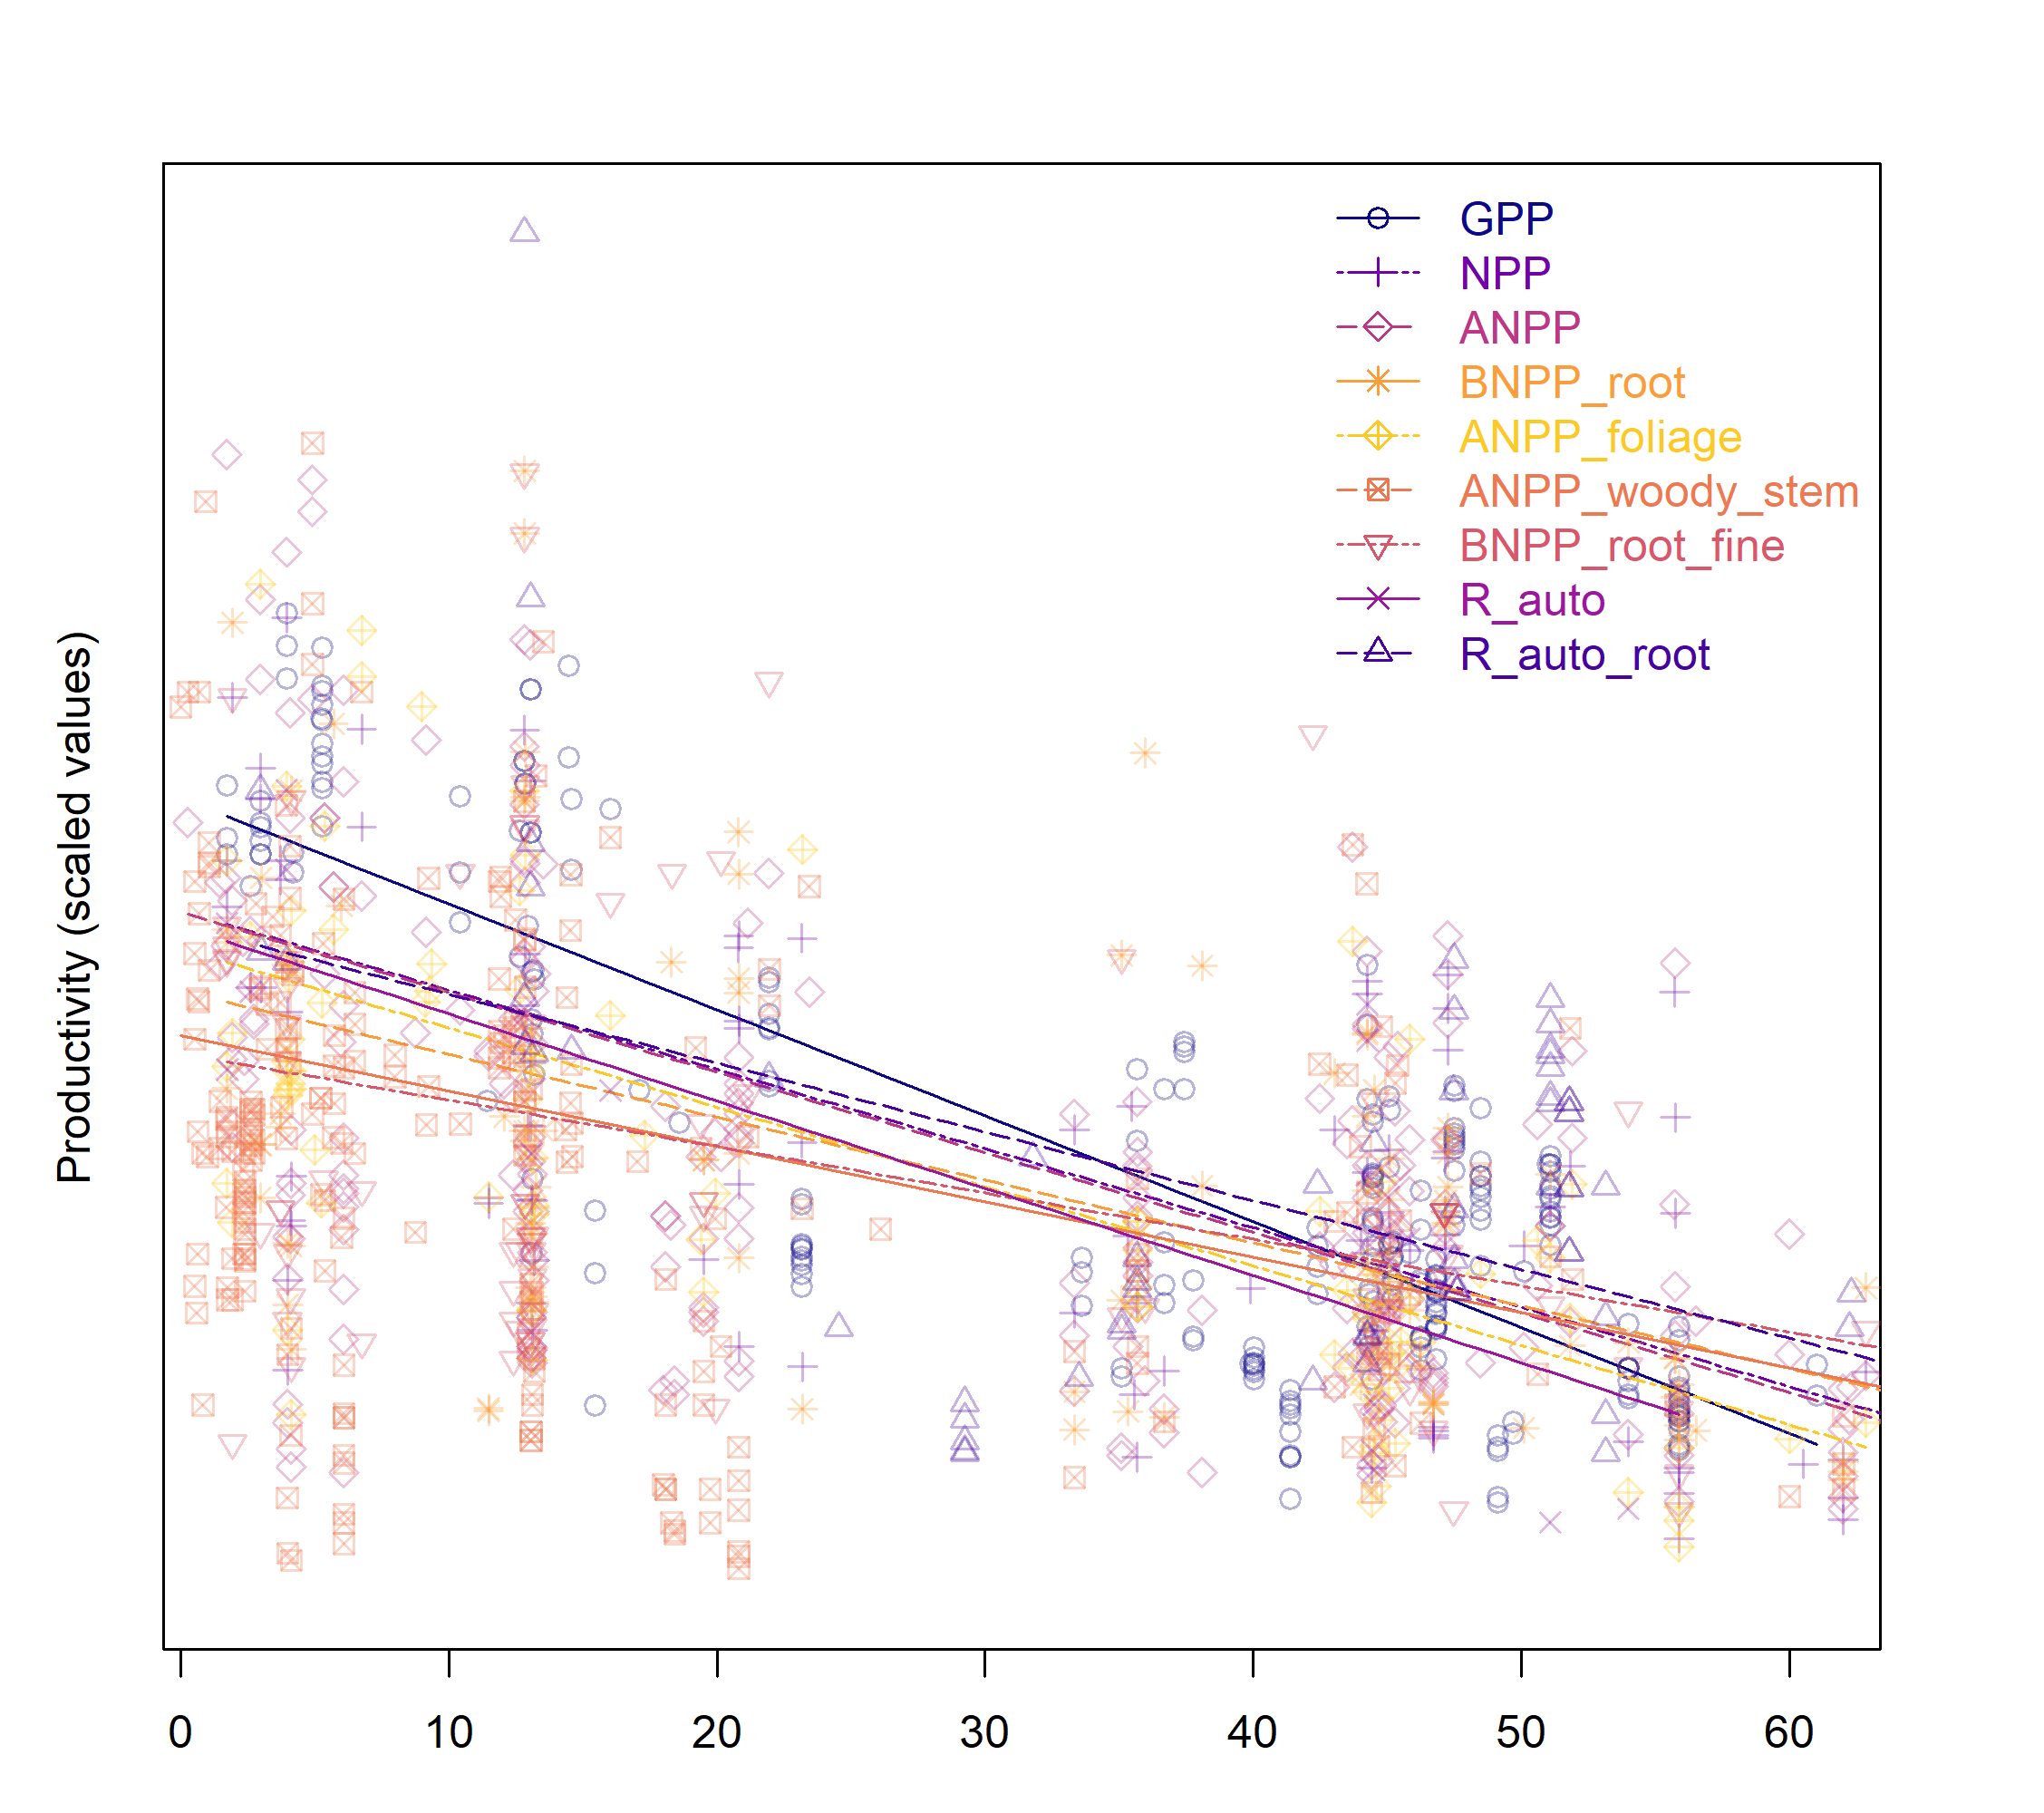
\includegraphics[width=1\linewidth]{effect_of_lat_transparent} \caption{Graphs to show primary productivity $(MgC~ha^-1~yr^-1)$ regressed against latitude. Lines of best fit are plotted according to the best model selected during analysis. All regressions are significant $(p<0.05)$.}\label{fig:unnamed-chunk-6}
\end{figure}

Latitude was a strong predictor for many of the carbon fluxes,
explaining 64\% of variation in GPP (n = 254, p\textless{}0.0001), 50\%
in NPP (n = 114, p\textless{}0.0001) and 45\% in ANPP (n = 259,
p\textless{}0.0001). For all fluxes, their relationship with latitude
was best predicted by the linear model.

\emph{Relationships and differences among fluxes.} In general, smaller
component fluxes summed approximately to larger fluxes across the
latitudinal gradient (fig. 3). That is, modelled estimates of GPP,
generated from the sum of NPP and R auto; NPP, generated from the sum of
ANPP and BNPP\textsubscript{root}; and ANPP, generated from the sum of
ANPP\textsubscript{foliage} and ANPP\textsubscript{woody}
\textsubscript{stem}, fell completely within the confidence intervals of
the regressions of field estimates of GPP, NPP and ANPP respectively.

bbl: here or in the discussion, note that this is a fairly stringent
test: it's easy for sub-fluxes not to sum up! (Extensive citations from
EC literature for example.)

\begin{figure}[H]
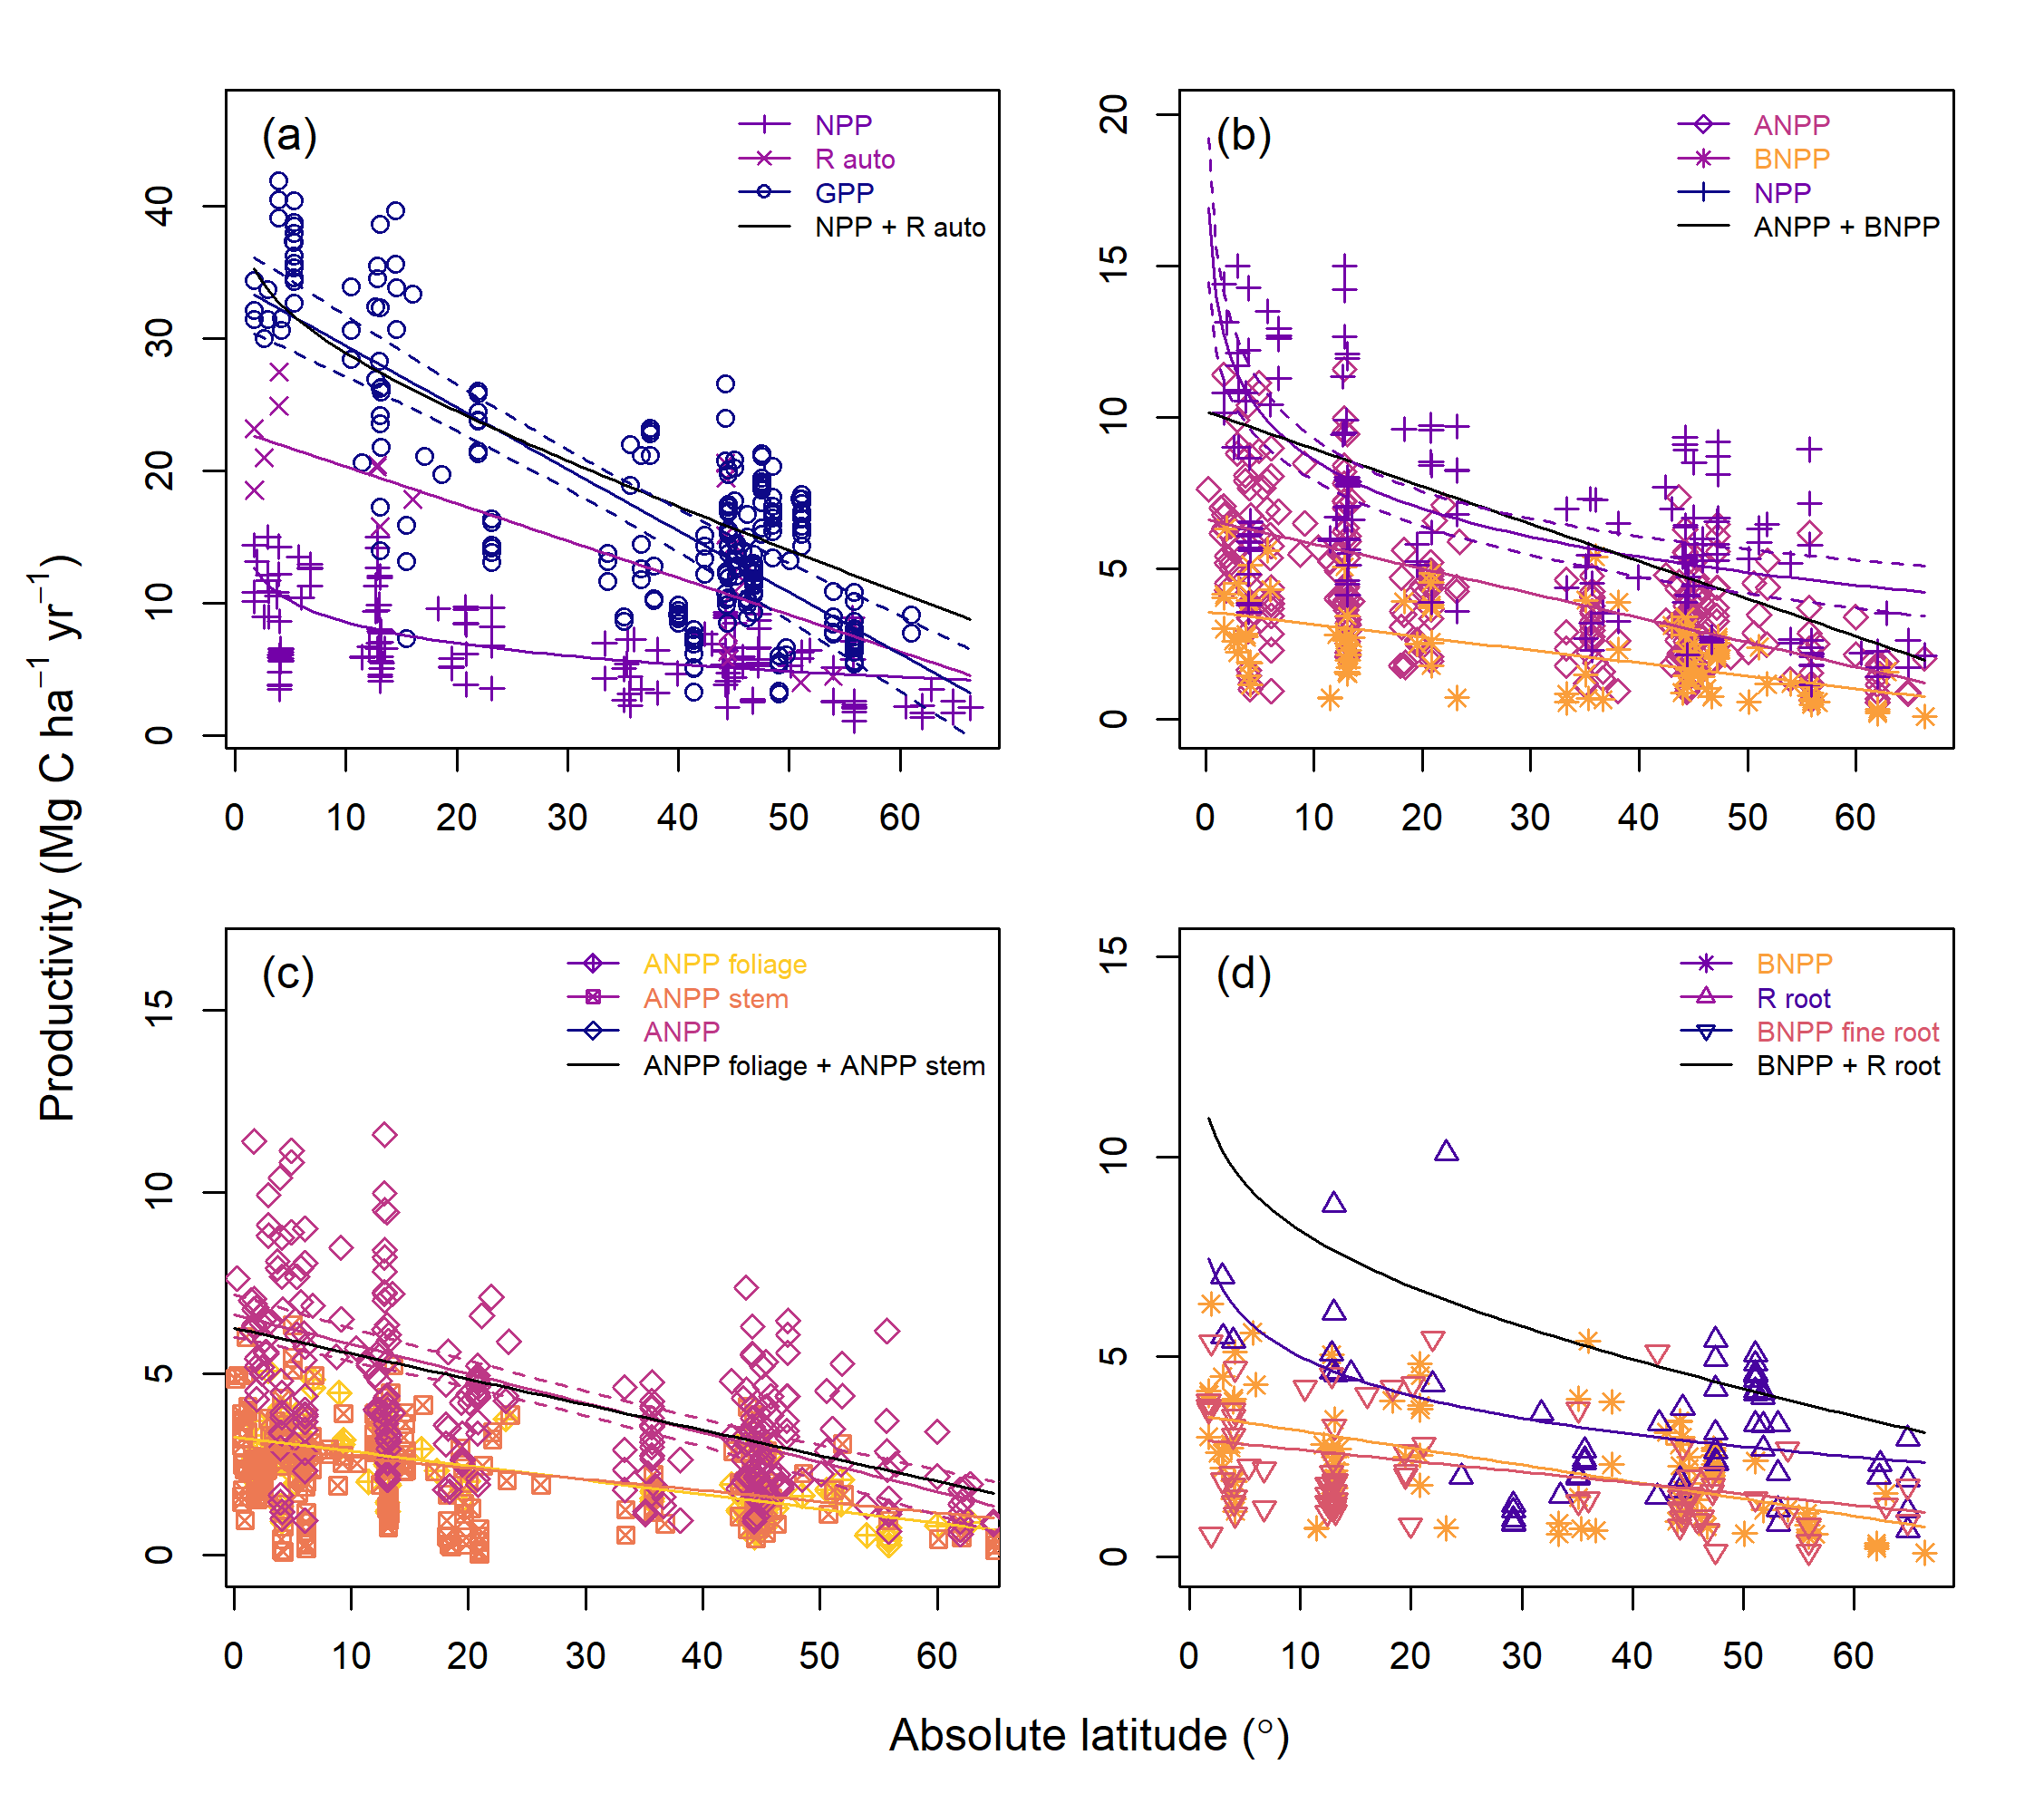
\includegraphics[width=1\linewidth]{combined_stacked} \caption{Graphs of primary productivity $(MgC~ha^-1~yr^-1)$ regressed against latitude. Lines of best fit are plotted according to the best model selected during analysis. All regressions are significant $(p<0.05)$. Plots 1 - 3 show two component fluxes; a larger flux, defined as the combination of the two component fluxes; and a modelled estimate of the sum of the two component fluxes. 95\% confidence intervals are plotted for the larger flux. Plot 4 shows three belowground fluxes, and a modelled estimate of the total belowground carbon flux}\label{fig:unnamed-chunk-7}
\end{figure}

We found no evidence that allocation between fluxes varied substantially
with latitude or climate. There were no significant results from
regressing ratios of carbon fluxes against latitude, or against any of
the climate variables.

\(R^2\) values were generally highest in the major fluxes, and decreased
in subsidiary fluxes (Supporting Information S2). Of the major fluxes,
R\textsubscript{auto} and GPP were the most strongly explained by
latitude and climate, with climate explaining at most 71\% of variation
in GPP, and 65\% in R\textsubscript{auto}. The proportion of variation
explained by climate and latitude decreased in NPP and ANPP, with
climate explaining at most 51\% of variation in NPP and 44\% in ANPP. Of
the major fluxes, BNPP\textsubscript{root} was the least well explained
by climate and latitude, with climate explaining at most 36\% of
variation.

With the exception of ANPP\textsubscript{foliage}, the proportion of
variation explained by climate and latitude in subsidiary fluxes was
much lower. Climate explained at most 24\% of the variation in
ANPP\textsubscript{woody} \textsubscript{stem}, 19\% in
BNPP\textsubscript{fine} \textsubscript{root}, and 27\% in
R\textsubscript{root}. In contrast, climate strongly explained variation
in ANPP\textsubscript{foliage}, with mean annual temperature explaining
58\% of variation. This pattern was also seen in the \(R^2\) values for
multivariate models.

\emph{How does productivity relate to MAT and MAP?} MAT and MAP are the
most commonly reported site-level climate variables, and much previous
research into the effect of climate on forest productivity has focused
on these as key climate variables. MAT was a significant
(p\textless{}0.05) and strong predictor of productivity for all carbon
fluxes tested, with all fluxes showing a linear increase with
temperature (fig. 5). We found no support for a saturation point of
productivity with temperature.

MAP was found to be a significant (p\textless{}0.05) but poor predictor
of productivity, explaining, with the exception of
R\textsubscript{auto}, at most 37\% of variation in carbon flux. For the
majority of fluxes productivity was best predicted by a polynomial
model. Productivity increased with precipitation, up until a saturation
point at between 3000 and 4000mm annual precipitation, above which
productivity started to decrease (fig. 5). The notable exception to this
was GPP: the model indicated that GPP continued to increase with
precipitation up to measures of at least 5000mm annually
(p\textless{}0.0001, \(R^2\) = 0.33. Data above this point was not
available, but the model trend indicated that the saturation point for
this model would be around 5000mm MAP.

There was a significant interactive effect between MAT and MAP for GPP,
BNPP\textsubscript{root}, BNPP\textsubscript{fine} \textsubscript{root},
ANPP, ANPP\textsubscript{woody} \textsubscript{stem}, and
R\textsubscript{root} (fig.4). There was a significant additive effect
for R\textsubscript{auto}. NPP and ANPP\textsubscript{foliage} showed no
significant interactive or additive effect.

For the variables which showed a significant interactive or additive
effect between MAT and MAP, no other climate variable, in combination
with MAT, significantly improved on that model. For NPP, there was a
significant interactive effect between MAT and water stress months, with
this model explaining nearly 5\% more variation in NPP than MAT alone.
However, for ANPP\textsubscript{foliage}, no multivariate model improved
on the univariate model including only MAT.

\begin{figure}[H]
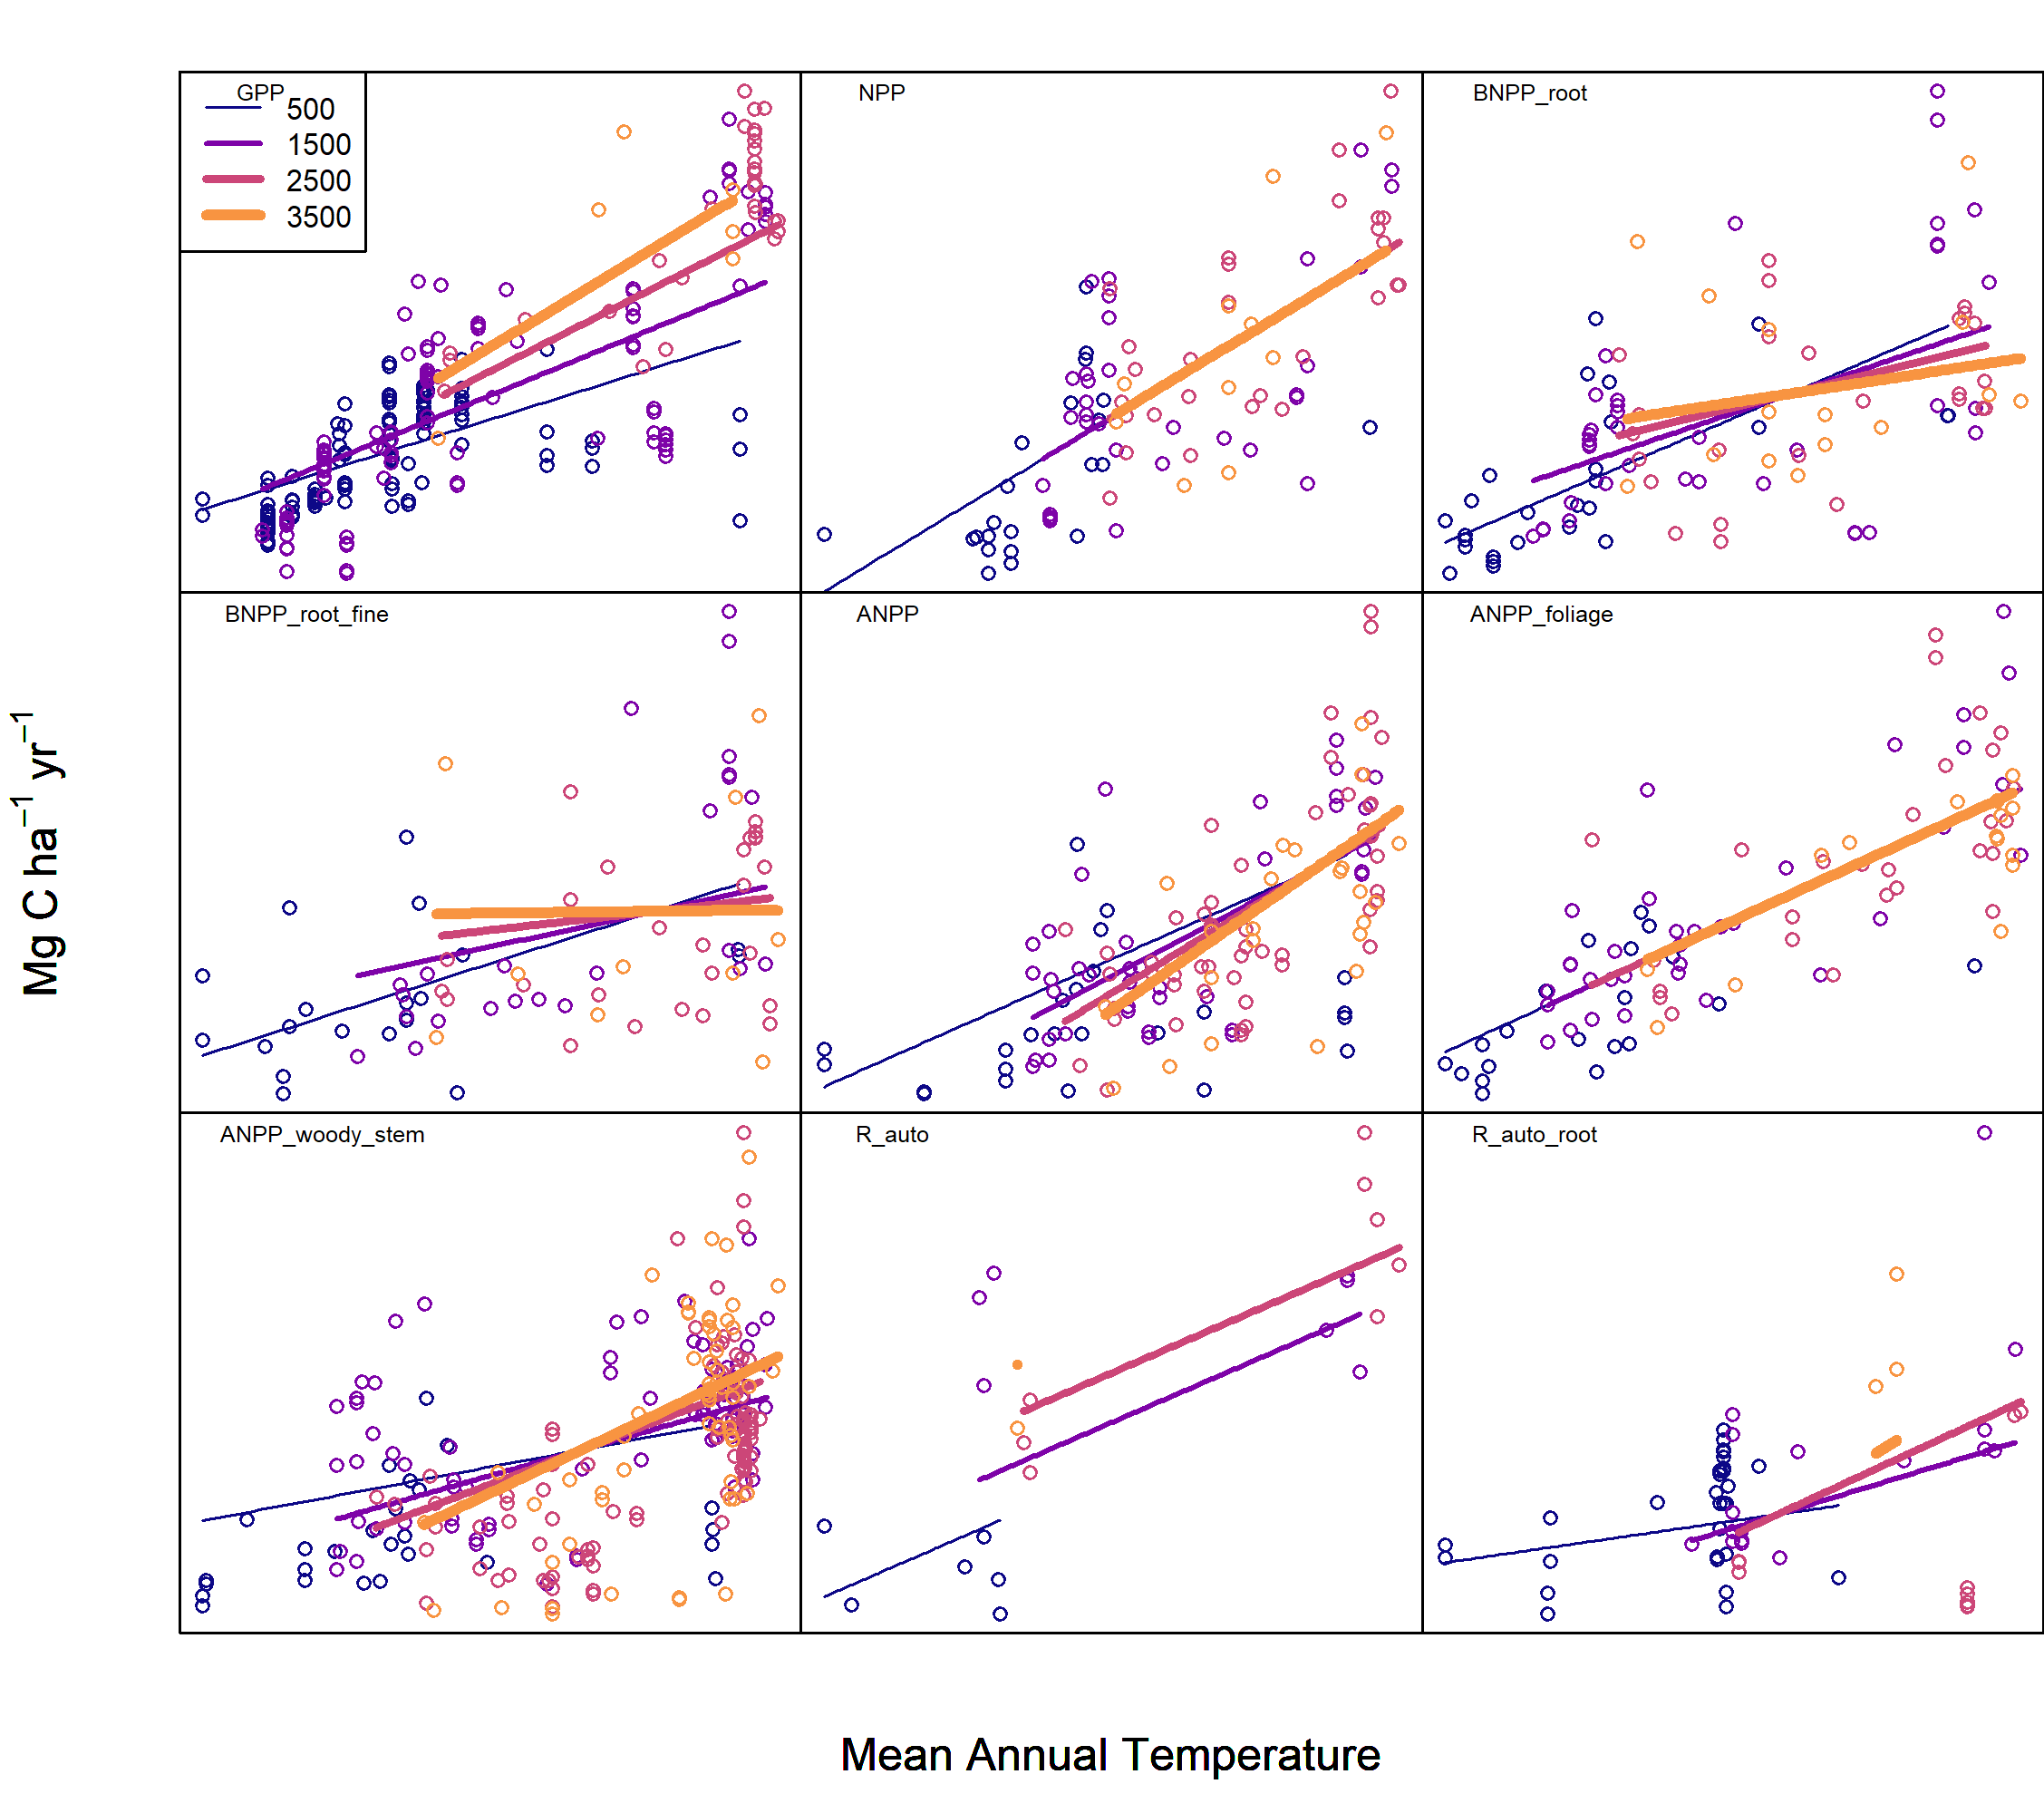
\includegraphics[width=1\linewidth]{mat_map_interaction} \caption{Plots of primary productivity $(MgC~ha^-1~yr^-1)$ regressed against mean annual precipitation. Points are grouped into bins of 0 - 1000, 1001 - 2000, 2001 - 3000, and >3000mm mean annual precipitation, and lines of best fit plotted for mean annual precipitation values of 500, 1500, 2500, and 3500mm. All regressions are significant $(p<0.05)$.}\label{fig:unnamed-chunk-8}
\end{figure}

\emph{How does productivity relate to other climate variables?} Our
results indicated that productivity was most strongly explained by
temperature at the global scale, with temperature-related climate
variables coming out as strong predictors of productivity. In addition
to MAT, temperature seasonality, annual temperature range, and annual
frost days were consistently identified as good predictors of
productivity across fluxes.

We found a significant relationship between productivity and potential
evapotranspiration for all fluxes. ANPP\textsubscript{foliage},
BNPP\textsubscript{fine} \textsubscript{root} and R\textsubscript{root}
increased linearly with PET; however, all other fluxes showed a
polynomial relationship with PET (fig. 5). We found strong evidence for
a saturation point or peak with PET: productivity tended to increase at
values below 1000mm, before saturating between 1200 and 1700mm. There
was also evidence that productivity begins to decrease at values above
1800mm PET.

Vapour pressure deficit was a significant predictor of productivity for
all fluxes. BNPP\textsubscript{fine} \textsubscript{root} showed a
linear relationship with vapour pressure deficit (\(R^2\) = 0.07,
p\textless{}0.05), but all other fluxes showed a polynomial relationship
(fig. 5). Productivity initially increased with vapour pressure deficit,
before saturating at around 0.8 kPa. At values above 0.8 kPa,
productivity began to decrease.

All fluxes, with the exception of R\textsubscript{root}, showed a
positive linear relationship with solar radiation. Solar radiation
explained a low proportion of variability in productivity for all
fluxes, explaining less than 20\% of the variation in each flux, with
the exception of R\textsubscript{auto} (\(R^2\) = 0.26,
p\textless{}0.05).

Of the climate variables tested, annual wet days, aridity, cloud cover,
mean diurnal temperature range, precipitation seasonality, maximum
vapour pressure deficit and water stress months were poor or
non-significant explainers of variation in productivity, explaining less
than 20\% of the variation in each of the carbon fluxes.

\begin{figure}[H]
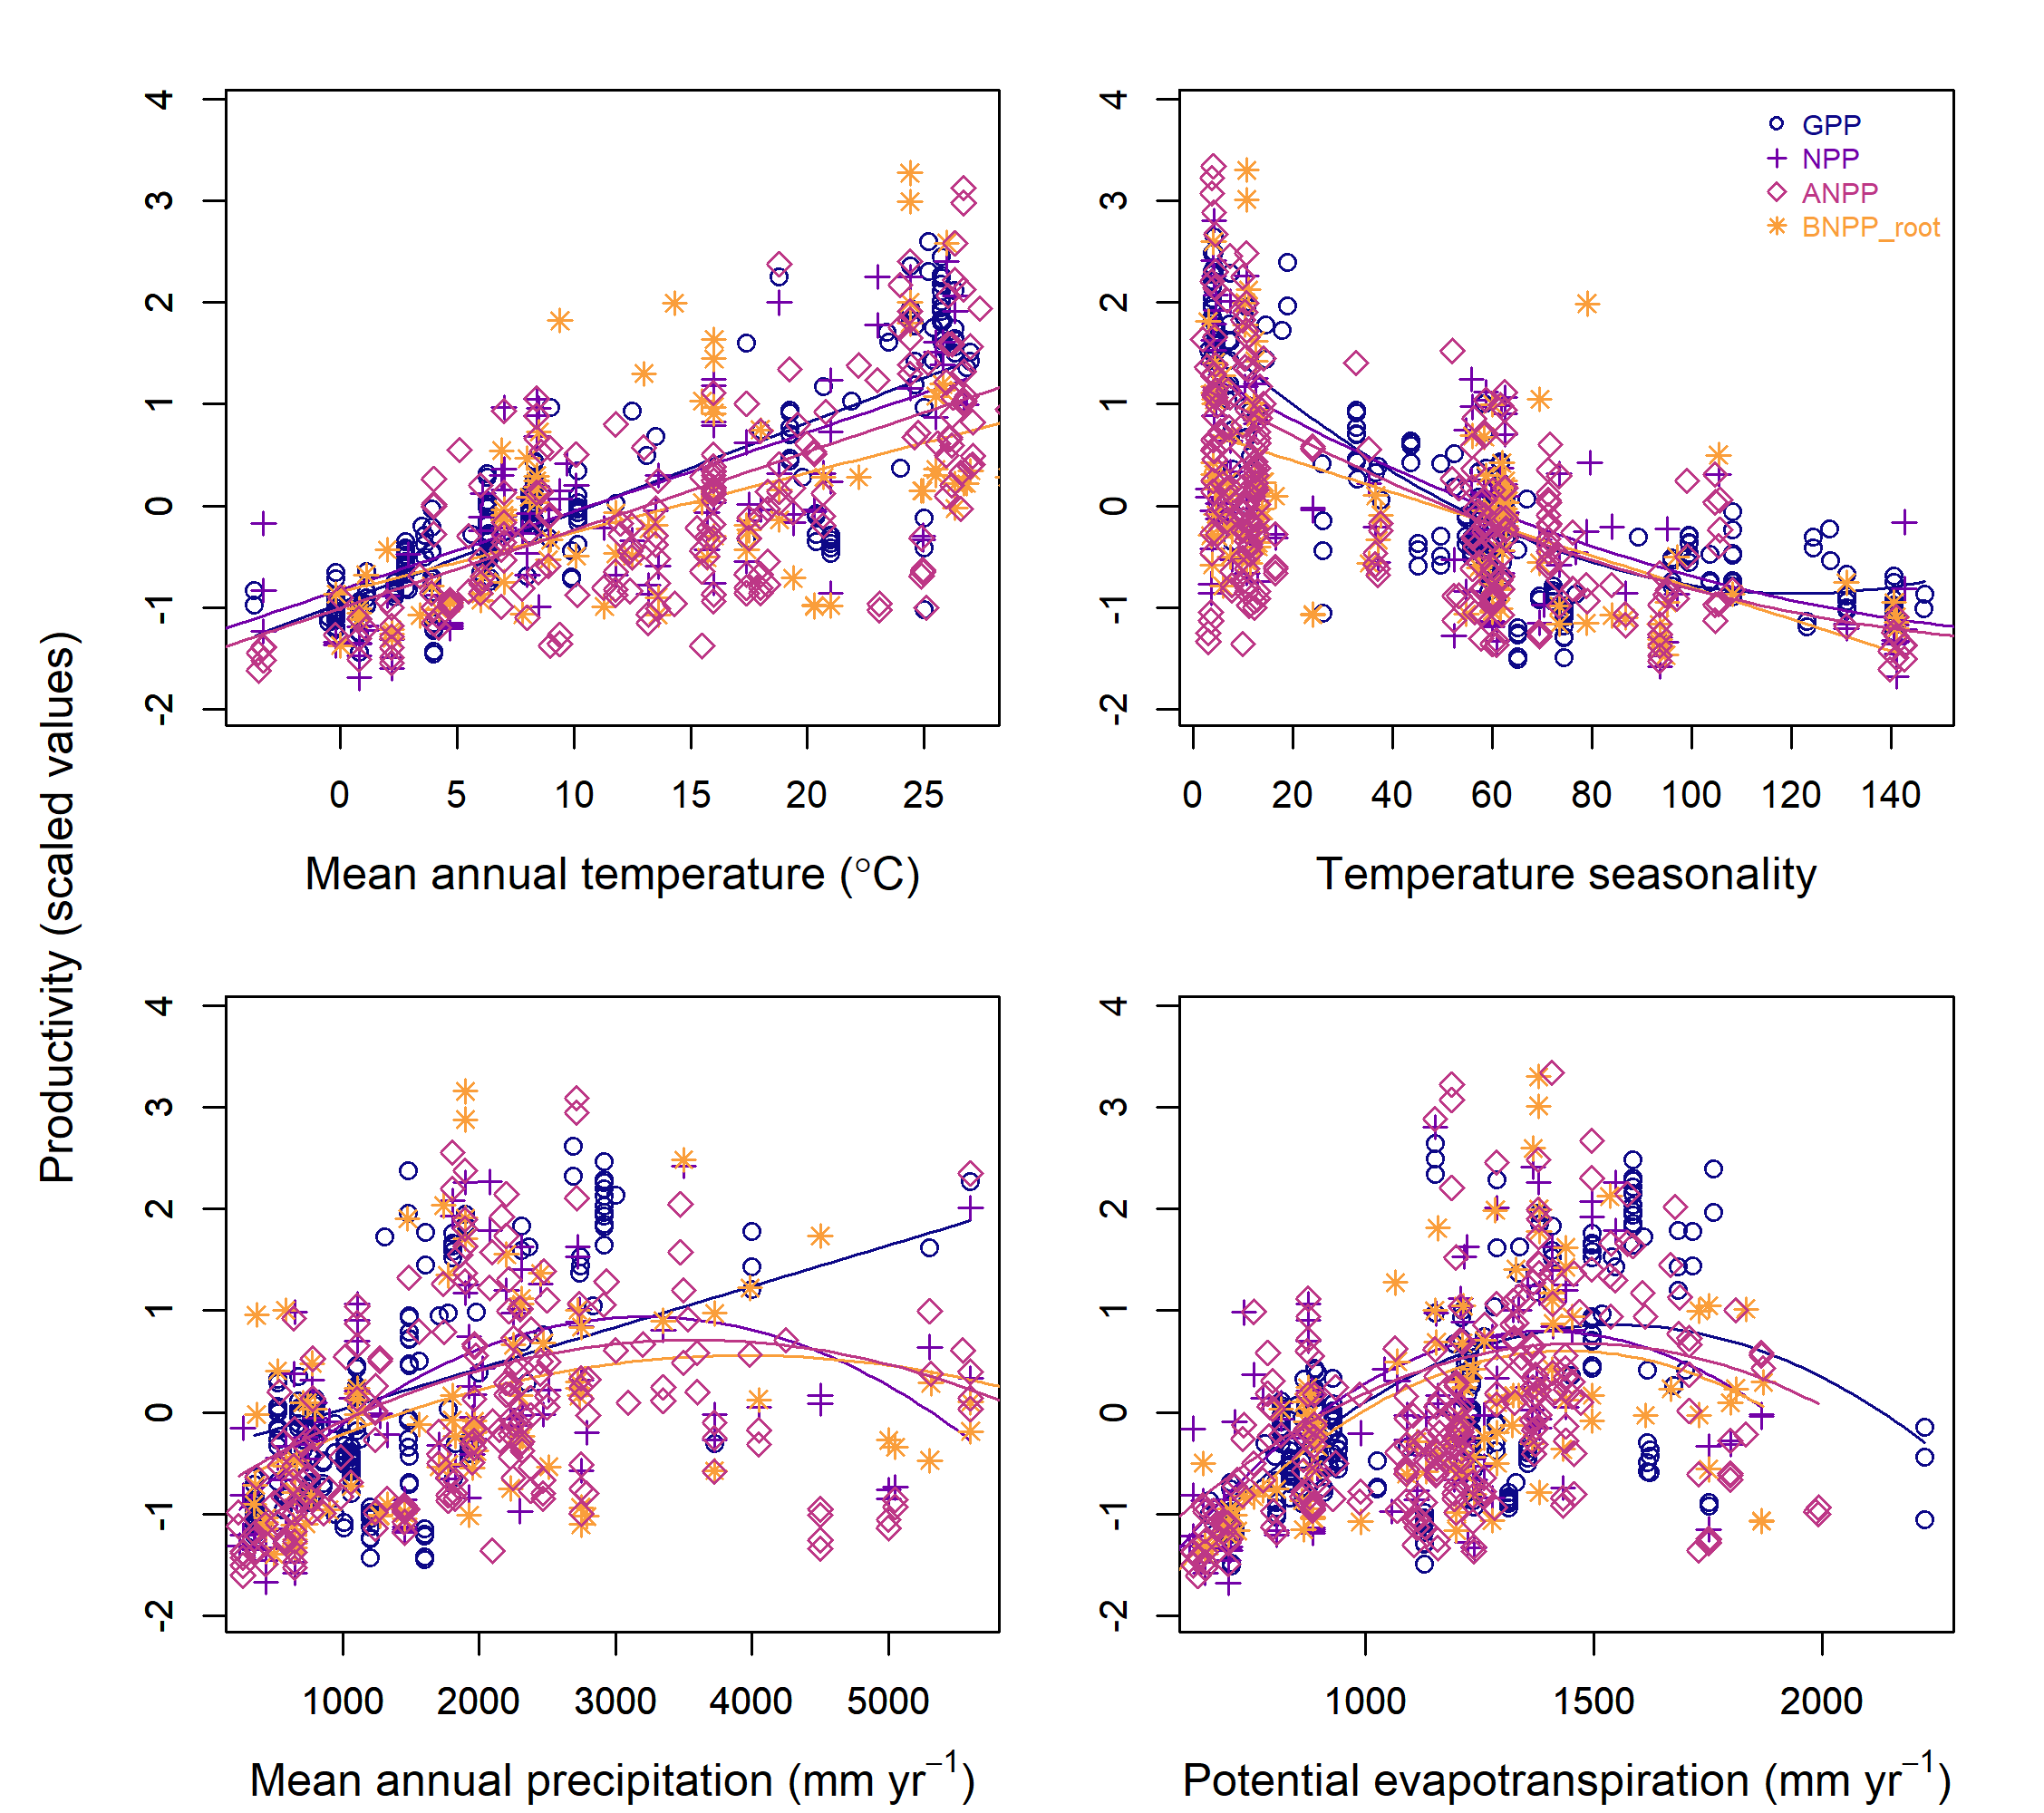
\includegraphics[width=1\linewidth]{combined_plots} \caption{Plots of primary productivity $(MgC~ha^-1~yr^-1)$ regressed against (a) mean annual temperature; (b) mean annual precipitation; (c) potential evapotranspiration, (d) vapour pressure deficit; (e) temperature seasonality; (f) length of growing season. Lines of best fit are plotted according to the best model selected during analysis. All regressions are significant $(p<0.05)$.}\label{fig:unnamed-chunk-9}
\end{figure}

\emph{What is the role of seasonality in explaining productivity?}
Temperature seasonality was a significant predictor of productivity.
GPP, NPP, ANPP, and R\textsubscript{root} exhibited a polynomial
relationship with seasonality (fig. 5). ANPP\textsubscript{foliage},
ANPP\textsubscript{woody} \textsubscript{stem} and R\textsubscript{auto}
decreased linearly with temperature seasonality. Temperature seasonality
was strongly correlated with annual temperature range, and, as expected,
all fluxes showed almost identical responses to it. Productivity was
highest where temperature seasonality = 0, and at an annual temperature
range of 15\(^\circ\)C or lower. In contrast, there was no significant
effect of precipitation seasonality on productivity.

We found a significant relationship between length of growing season and
productivity, with all fluxes showing a linear increase in productivity
with length of growing season (fig. 5). Length of growing season was a
strong predictor of productivity, explaining 51\% of variation in GPP,
39\% of variation in NPP, and 34\% of variation in ANPP, but it was not
identified as a stronger predictor than MAT for any of the fluxes
analysed.

\emph{Within the growing season, how does productivity vary with
climate?} Within growing season months, we found that climate had a much
weaker effect on productivity. For each of temperature, precipitation,
PET, and solar radiation, we found a small effect of climate for certain
carbon fluxes. There was a small increase in productivity with
temperature and precipitation for ANPP (with temperature \(R^2\) = 0.10,
p\textless{}0.001; with precipitation \(R^2\) = 0.04, p\textless{}0.05)
and ANPP\textsubscript{foliage} (with temperature \(R^2\) = 0.16,
p\textless{}0.01; with precipitation \(R^2\) = 0.09, p\textless{}0.05).
Productivity increased with solar radiation for GPP (\(R^2\) = 0.21,
p\textless{}0.001), NPP (\(R^2\) = 0.21, p\textless{}0.001), BNPP
(\(R^2\) = 0.16, p\textless{}0.001) and BNPP\textsubscript{fine}
\textsubscript{root} (\(R^2\) = 0.12, p\textless{}0.01), and with PET
for GPP (\(R^2\) = 0.15, p\textless{}0.01), NPP (\(R^2\) = 0.18,
p\textless{}0.01), BNPP (\(R^2\) = 0.23, p\textless{}0.0001),
BNPP\textsubscript{fine} \textsubscript{root} (\(R^2\) = 0.11,
p\textless{}0.05), and ANPP\textsubscript{woody} \textsubscript{stem}
(\(R^2\) = 0.06, p\textless{}0.05).

\subsubsection{Discussion}\label{discussion}

We used a large global database (ForC), containing an unprecedented
amount of data representing all major forest types (Fig. 1) and the nine
most significant forest autotrophic carbon flux (FACF) variables (Table
2), to comprehensively explore how C cycling in mature, undisturbed
forests varies with latitude and climate on a global scale. We test a
suite of hypotheses, including many previously posed (Table 1),
standardising for factors that have not always been controlled for
(\emph{e.g.}, stand age, flux components measured) to gain a stronger
understanding of climatic effects on FACF.

bbl: Most of these two paragraphs (following) just restate the results.
Honestly I would remove them enitrely, but at the very least, condense
into a single paragraph.

We show that, across all nine FACF variables analyzed, C cycling
decreases linearly with latitude (\emph{H1.1}; Figs. 2-3)--a finding
that confirms multiple previous studies (\textbf{REFS}) but contradicts
the idea that productivity of temperate forests rivals that of tropical
forests (\emph{H1.1.alt}; \textbf{REFS}). The FACF variables increase in
proportion to one another (\emph{H1.2}), with no differences in
allocation detectable at this global scale and with component fluxes
summing appropriately to larger fluxes (Fig. 3), indicating no major,
systematic omissions or overestimations of flux components. However, we
did detect a tendency for greater variability among subsidiary C fluxes
(e.g., \emph{\(ANPP_{woody}\)}, \emph{\(BNPP_{fine.root}\)}; Fig. 2;
\textbf{some SI table?}).

\textbf{Climate explains a significant proportion of variation in all C
fluxes analyzed} (albiet less for subsidiary fluxes), with temperature
variables the best predictors of FACF at this global scale (Figs. 4-5).
While other climate variables are significant predictors of FACF
(\emph{H3}), none of them improve on the explanatory power of
temperature-related variables in general or MAT specifically (Fig. 5).
Water availability is an important factor in explaining FACF on a global
scale: we find a positive influence of precipitation at low MAP, with
saturation at higher levels of MAP (Fig. 5b) and a significant
interaction between MAT and MAP for seven of the nine variables analyzed
(Fig. 4). Temperature seasonality and growing season length are closely
correlated with MAT and are strong predictors of FACF (\emph{H4}; Fig.
5e-f), though growing season length doesn't improve upon MAT as a
predictor. Within the growing season, the influence of climate on C
cycling is smaller but still significant for a number of carbon fluxes
(\emph{H5}; \textbf{some SI table?}). These findings clarify the big
picture of how FACF varies with latitude and climate on a global scale.

Past studies have differed in their conclusions regarding the
relationship between productivity and latitude or its correlates (Table
1, \emph{H1}; \textbf{REFS})--quite possibly because of lack of
standardization with respect to stand age and disturbance history. Our
findings indicate that, among mature, undisturbed stands, FACF is
unambiguously highest in the tropical regions, and the relationship is
approximately linear (Figs. 2-3). This contrasts with suggestions that
productivity of temperate forests is similar to that of tropical forests
(\textbf{REFS}). Temperate forests tend to be younger than tropical
forests (\textbf{REF}), so analyses comparing across latitudinal
gradients without controlling for stand age risk confounding age with
biome effects (\href{http://pure.iiasa.ac.at/id/eprint/15361/}{Poulter
et al. 2018-DOI:10.1594/PANGAEA.889943}; Potapov et al. 2008. Mapping
the World's Intact Forest Landscapes by Remote Sensing. Ecology and
Society 13 (2), 51. ). In addition, because C allocation varies with
stand age \citep{de_lucia_forest_2007} (\textbf{See Nobby's comment in
manuscript-draft\_NK.pdf}), age differences may introduce systematic
biases into analyses of FACF across latitude or global climatic
gradients. For example, woody productivity tends to be higher in rapidly
aggrading secondary stands than in old-growth forests, where
proportionally more C is allocated to respiration (** Nobby AFM paper:
Understanding the controls over forest carbon use efficiency on small
spatial scales: Effects of forest disturbance and tree diversity**)
{[}*purpose for respiration/ other compenents (\textbf{See Nobby's
comment in manuscript-draft\_NK.pdf}){]}.

We show that FACF are broadly consistent in their responses to climate
drivers on the global scale (with the exception of some differences in
MAT-MAP interactions; Fig. 4), with no major trends in C allocation
among the variable pairs tested (Table 1, \emph{H1}; Fig. 2;
\textbf{Some SI table}). Although variation in allocation has been
observed along gradients of elevation \citep{moser_elevation_2011} and
water availability \citep{newman_above-_2006}--along with non-climatic
axes of stand age \citep{litton_carbon_2007}, nutrient availability
\citep{litton_carbon_2007, gill_belowground_2016}, and forest structure
\citep{taylor_greater_2019}--variation in relation to climate is not
apparent at the global scale within ForC, which contains the bulk of
relevant data. Our conclusion, then, is that hypothesized gradients in
allocation along global climate gradients cannot currently be supported
for mature forests, although data quantity and standardization is
currently insufficent to rule out the possibility that such trends
exist.

bbl: remove this sentence? Of particular interest and significance are
the relationships amongst \(GPP\), net primary productivity (\(NPP\) and
its components, particularly \(ANPP_{woody-stem}\)), and respiration
(\(R_{auto}\) and components). There have been suggestions that tropical
forests tend to have low carbon use efficiency (\(CUE\)=
\(NPP\)/\(GPP\)=(\(GPP\)-\(R_{auto}\)/\(GPP\)), which are based on
observations of low \(CUE\) in old-growth tropical forests relative to
(mostly younger) extratropical forests
\citetext{\citealp{de_lucia_forest_2007}; \citealp[\href{https://www.researchgate.net/publication/227837530_The_productivity_metabolism_and_carbon_cycle_of_tropical_forest_vegetation}{Malhi
2012};][]{anderson-teixeira_carbon_2016}}, but our analysis suggests
that these low values might more appropriately be attributed to the fact
that these forests are old than to their tropical climate. Indeed,
\(CUE\) is known to decline with forest age
(\citep{de_lucia_forest_2007};
\href{https://academic.oup.com/treephys/article-abstract/39/8/1473/5423351?redirectedFrom=fulltext}{Collalti
\& Prentice 2019}) but appears to be roughly independent of \(GPP\)
\citep{litton_carbon_2007}. Among our sites with relevant data, there is
indication that CUE or \(ANPP_{woody-stem}\)/\(GPP\) increase with
latitude (\textbf{some SI table}). Additional measurements with careful
methodological standardization across a consistent set of mature forest
sites will be necessary to determine whether any climate-driven
gradients in allocation exist at the global scale.

One interesting observation was that climate tends to explain more
variation in the major fluxes (\(GPP\), \(NPP\), \(R_{auto}\) - latitude
\(R^2\ge\) 48\%) than in subsidiary fluxes (latitude \(R^2\)
\textless{}27\% for \(BNPP_{fine.root}\),
\(R_{auto-root}\),\(ANPP_{woody-stem}\)) (Fig. 2; \textbf{some SI
table?}). There are two, non-exclusive, potential explanations for this.
First, it may be that methodological variation is larger relative to
flux magnitude for some of the subsidiary fluxes. Belowground fluxes in
particular are difficult to quantify, and measurement methods for the
belowground fluxes considered here may be measured through fundamentally
different approaches (\emph{e.g.}, minirhizotrons, ingrowth cores, or
sequential coring for \(BNPP_{root-fine}\); root exclusion, stable
isotope tracking, or gas exchange of excised roots for
\(R_{auto-root}\)), and sampling depth is variable and often
insufficient to capture the full soil profile. \(ANPP_{woody-stem}\),
which is also poorly explained by latitude or climate, is more
straightforward to measure but is subject to variability introduced by
differences such as biomass allometries applied and minimum plant size
sampled (bbl: cite e.g.~Huntzinger?). However, methodological variation
and uncertainty affect all of fluxes considered here--not necessarily
any less than the aforementioned, and some of the larger fluxes that
vary more strongly with respect to climate (\(ANPP\), \(NPP\)) are
estimated by summing uncertain component fluxes. Second, differences
among variables in the proportion of variation explained by climate may
be attributable to more dicrect climatic control over \(GPP\) than
subsidiary fluxes. That is, subsidiary fluxes may be shaped by climate
both indirectly through its influence on \(GPP\) and respiration and
directly through any climatic influence on C allocation, as well as by
many other local- and regional-scale factors (\textbf{REFS}).

The latitudinal gradient in FACF (Figs. 2-3) is driven primarily by
temperature-related climate variables, and secondarily by moisture
availability (Table 1, \emph{H2-H3}; Figs. 4-5). Because many climate
variables co-vary across the latitudinal gradient, because climatic
drivers affect forest carbon flux on much shorter time scales than can
be captured by annual climate summary variables, and because both
climatic conditions and C flux vary intra- and inter-annually around the
long-term means, it is not appropriate to attempt to identify any one
mean annual climate variable as a mechanistic driver of FACF. However,
it remains informative to consider these relationships. We find that
temperature-related climate variables (\(MAT\), temperature seasonality,
\ldots{}\textbf{LIST}) explain the highest proportion of variability in
productivity, and among these, \(MAT\) is generally the best
predictor--perhaps because site-specific MAT is recorded for the
majority of sites in ForC, whereas other variables are extracted from
global gridded data products (Table S1\textbf{?}). The effects of
temperature are modified by moisture availability, with reduced FACF
under hot and dry conditions (\emph{i.e.}, high PET, high deficit; Fig.
5c-d) and sometimes under very high precipitaiton (Figs. 4, 5b).
Negative effects of very high precipitation on FACF have been previously
observed (\textbf{REFS}) and are attributable to nutrient and light
limitations (\textbf{REFS}) Thus, although temperature and water
availability jointly and interactively drive global-scale patterns of
FACF.

bbl: this seems really interesting and novel, consider expanding the
following paragraph

FACF is reduced by temperature seasonality (Table 1, \emph{H4}; Fig.
5e), and productivity is shut down during cold- or dry- dormant seasons.
To account for this, a number of analyses seeking to characterize
global-scale effects of climate on productivity have examined the
relationship of FACF per month of the growing season with growing season
climatic conditions (Table 1, \emph{H5}; \textbf{REFS}). We found that
the sort of simple metric needed to define growing season at a global
scale was uncertain for temperature and problematic for moisture
(\textbf{WORK ON THIS}). A temperature-defined growing season length had
stong positive correlation with FACF (Fig. 5f), but explained less
variation than \(MAT\). Dividing FACFs by growing season length to yield
FACF per growing season month removed the majority of climate-related
variation, supporting the idea that the latitudinal gradient in FACF is
attributable more to shorter growing seasons at high latitudes than to
inherently lower rates of photosyntheiss or respiration by high-latitude
forests (\emph{{[} Enquist et al. 2007 GCB- but check{]}}). However,
there remained a number of significant correlations with growing season
climatic conditions, suggesting that climatic conditions remain
influential within the growing season. We conclude that while correcting
for growing season length takes analyses a step closer to mechanistic
linkage of instantaneous C flux rates to environmental conditions, it
remains very crude relative to the the timescales on which climate
affects plant metabolism and does not advance statistical predictive
power. Rather, mechanistic accounting for climatic effects on global
productivity patterns requires models representing physiologically
meaningful timescales (\emph{e.g.}, \textbf{refs}).

Our analysis clarifies how FACF varies (bbl: is FACF singular or plural?
Be consistent) with latitude and climate on a global scale, with some
important implications for how forest carbon cycling relates to climate
and, by extension, how it is likely to respond to climatic warming. We
find no support for non-linear trends in mature forest C cycling with
respect to latitude or \(MAT\), and no distinct trends in C allocation
across the global scale (Fig. 3). The implication is that under warmer
conditions with similar moisture availability--and within the
temperature range to which forest communities are adapated and
acclimatized--higher temperatures result in a generalized acceleration
of FACF, with no major shifts in C allocation among subsidiary fluxes.
Of course, actual climatic changes will result in very different sets of
conditions than represented across geographic gradients in climate, but
our analysis clarifies how carbon cycles through contemporary forest
ecosystems. As we enter a period of accelerating climatic change,
understanding of the fundamental climatic controls on FACF sets a
foundation for understanding patterns of change. \textbf{{[}work on
this{]}}

\subsubsection{Acknowledgements}\label{acknowledgements}

Scholarly Studies ForestGEO Compilation of the ForC database was
originally funded by DOE

\bibliography{library.bib,packages.bib}


\end{document}
